\documentclass{article}
\usepackage{color}

\usepackage{paratype}
\usepackage[T1]{fontenc}

\usepackage{graphicx}
\graphicspath{{../images/tape_storage_element/}}

\usepackage[top=2cm, bottom=2cm, left=2cm, right=2cm]{geometry}
\setlength{\parindent}{0pt}
\setlength{\parskip}{1em}
\title{The tape Storage Element---Integrating CTA into the data archiving chain of CERN}
\author{Eric Cano \and Andreas Peters \and Giuseppe Lo Presti \and Luca Mascetti \and Steven Murray  \and Sebastien Ponce}

\begin{document}

\maketitle

\section{A brief introduction to CTA and the tape Storage Element}

CTA stands for the \textbf{C}ASTOR/\textbf{C}ERN \textbf{T}ape \textbf{A}rchive.  CTA is an asynchronous disk to tape, tape to disk transfer engine that schedules transfers with the aim of maximising the efficient use of tape hardware.  The inception of CTA came from the maintenance phase of CASTOR, the \textbf{C}ERN \textbf{A}dvanced \textbf{STOR}age management system.  CASTOR is a \textbf{H}ierarchical \textbf{S}torage \textbf{Ma}nagement (HSM) system developed at CERN that is responsible for archiving the custodial copy of physics data generated by the \textbf{L}arge \textbf{E}lectron \textbf{P}osition collider (LEP) experiments of the past and the \textbf{L}arge \textbf{H}adron \textbf{C}ollider (LHC) experiments of today and the future.

The physics programme of the LHC is divided into 3 physics runs.  Run 1 was from the beginning of 2010 through to the middle of 2012.  Run 2 is currently ongoing, having started in mid 2014 and will continue through to mid 2017.  Run 3 is planned to start in mid 2018 and continue through to mid 2021.  CASTOR will cope comfortably with the data taking demands of physics run 2 where approximately 45 petabytes of data shall be archived. Run 3 is expected to generate between 50 and 100 petabytes, with a figure near to 100 petabytes being the most likely.  The code and data CASTOR uses to schedule the efficient use of tape hardware is scattered over several of the components that make up CASTOR.  This scattering will make it difficult to adapt CASTOR to the data archiving requirements of LHC physics run 3 and it will definitely increase the reaction times of developers adapting the system to unforeseen problems during the run.

CTA will address LHC physics run 3 by gathering all of the code and data required to schedule tape hardware into a single modular component.  Being able to schedule tape hardware is not enough to construct a cleanly decoupled storage module.  External systems using the module will wish to copy data files to and from it synchronously which is in direct conflict with the asynchronous nature of tape hardware.  The external systems will also need to see a single namespace for the files being archived.  To conclude, CTA will need to be encapsulated within a storage module that also contains a disk-based staging area for tape and the necessary code and data to work with an archive namespace.  From now on this module will referred to as a tape Storage Element where the concept of Storage Element has been borrowed from the nomenclature of the LHC computing Grid.

\newpage
\section{Reasons for developing CTA and the tape Storage Element}
The following list gives the many reasons for developing CTA and the tape Storage element:
\begin{itemize}
  \item Simplify the CERN archive solution by profiting from the evolution of tape access:
  \begin{itemize}
  	\item Away from random access.
  	\item Towards bulk archival and retrieval.
  \end{itemize}
  \item The CASTOR namespace will not cope with the user request rate of LHC run 3.
  \item The future namespace technology of the DSS group should be able to store 50 billion files.
  \item There should be only one disk staging technology as opposed to having both EOS and CASTOR.
  \item Reduce the time and effort required to change the tape hardware scheduling logic by putting all of the data it requires in one place.
  \begin{itemize}
  	\item Hardware catalogue, queues, policies and constraints.
  	\item Global and consistent view.
	\item No scheduling decisions based on partial information.
	\item Simple and powerful platform for future improvements.
	\item Self-contained unit.
  \end{itemize}
  \item Provide EOS with direct access to tape.
  \item Open the door for reducing the number of disk layers between users and tape.
\end{itemize}

\newpage
\section{The architecture of CTA}
CTA is a disk to tape, tape to disk transfer engine.  CTA schedules these transfers to maximise the efficiency of the underlying tape hardware.  CTA has no disk storage of its own.  The scheduling logic of CTA assumes that the disk storage it interacts with will be able to provide adequate bandwidth to keep tape drives saturated most of the time. One of the design constraints of CTA is to avoid vendor lock in by using open source software solutions.  The following diagram shows a very simplified view of the architecture of CTA.

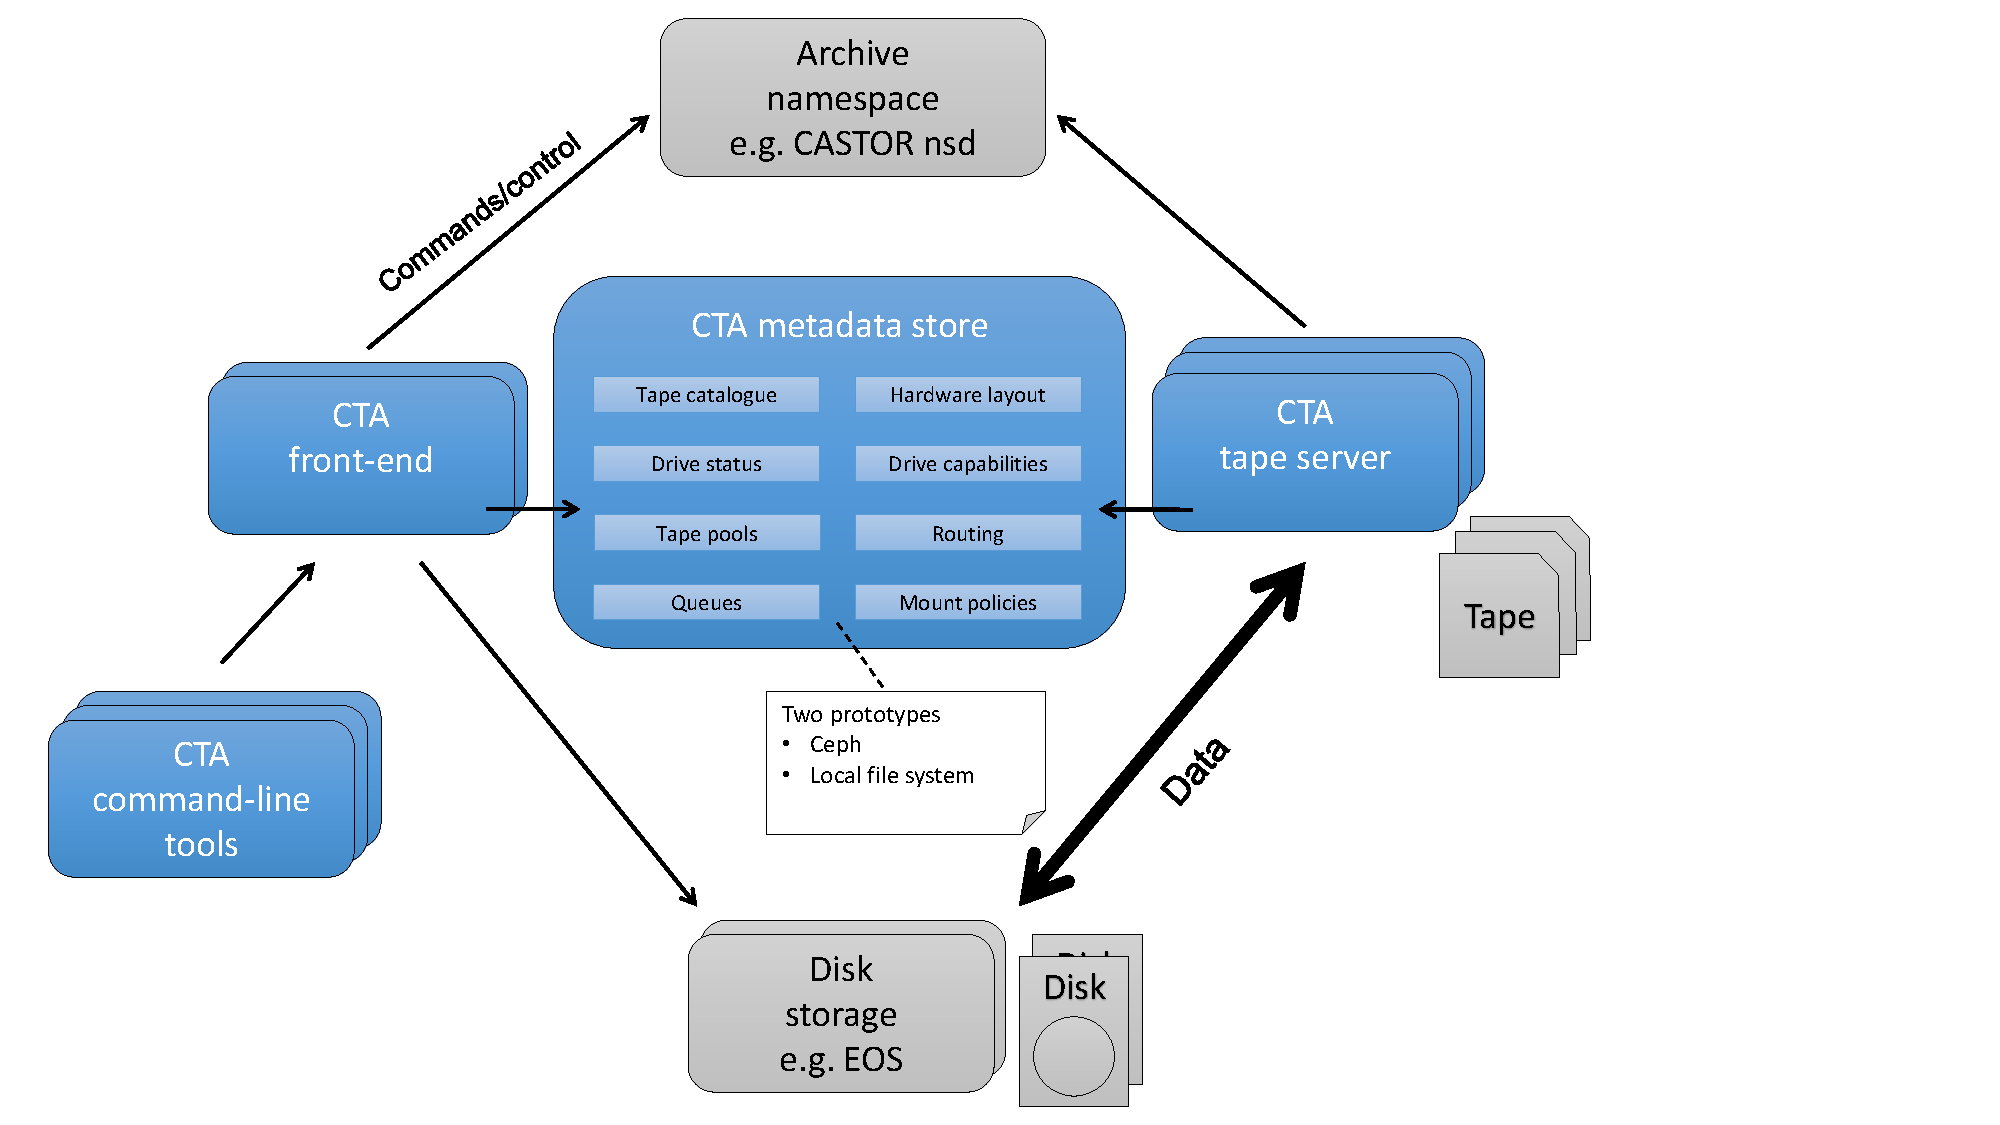
\includegraphics[width=\linewidth]{cta_architecture_simple}

CTA is composed of a set of command-line tools, one or more front-ends, a central metadata store and one or more tape servers.  CTA requires but does not provide an archive namespace and one or more disk-based storage systems.

The central metadata store can be viewed as a blackboard of work to be done by the tape servers.  Users run command-line tools that send requests to the front-ends which in turn write/queue those requests within the central metadata store.  The tape servers pull the requests from the store at the most appropriate moments in time in order to make efficient use of the underlying tape hardware.  Please note that a user of CTA will most probably be another system as opposed to an end user.

\newpage
\section{Problem dimensions}
The following list describes the dimensions of the future archival solutions based on empirical data collected from the current archive system used at CERN, namely CASTOR.
\begin{itemize}
	\item Peak performance of CASTOR tape that was sustained over 2 months
	\begin{itemize}
		\item 83 million files, 25 Petabytes per month
		\item Average file size = 300 Megabytes
		\item Average user request rate = 34 Hz
		\item Peak user request rate = 70 Hz
	\end{itemize}

	\item Current data rate of CASTOR is approximately 5 times less than the observed 2 month peak
	\begin{itemize}
		\item 6 Petabytes per month
		\item Average file size = 300 Megabytes
		\item User request rate = 8 Hz
	\end{itemize}

	\item Target user request rate
	\begin{itemize}
		\item Target one order of magnitude greater than peak performance
		\item 350 Hz average
		\item 700 Hz peak
	\end{itemize}
\end{itemize}

\section{How users interact with EOS and CASTOR}
\subsection{How LHC experiments transfer DAQ data to the CERN computing centre}
The following table lists how the four LHC experiments transfer data from the DAQ systems running in their experimental areas to the CERN computing centre.

\begin{tabular}{|l|l|l|}
	\hline
	Experiment & IT entry-point & DAQ to IT transfer mechanism \\
	\hline
	\hline
	ALICE      & CASTOR         & Standard copy using xrdcp    \\
	\hline
	ATLAS      & EOS            & Standard copy using xrdcp    \\
	\hline
	CMS        & EOS            & Standard copy using xrdcp    \\
	\hline
	LHCb       & CASTOR         & FTS + SRM + GridFTP          \\
	\hline
\end{tabular}


\subsection{How LHC experiments transfer data between EOS and CASTOR}
The following table lists how the four LHC experiments transfer data between EOS and CASTOR.

\begin{tabular}{|l|l|l|}
	\hline
	Experiment & Framework & Transfer mechanism                                          \\
	\hline
	\hline
	ALICE      & AliEn     & XRootD 3\textsuperscript{rd} party copy                     \\
	\hline
	ATLAS      & RUCIO     & FTS + CASTOR SRM + GridFTP                                  \\
	\hline
	CMS        & PhEDEx    & FTS + CMS plug-in + XRootD 3\textsuperscript{rd} party copy \\
	\hline
	LHCb       & DIRAC     & FTS + EOS SRM + CASTOR SRM + GridFTP                        \\
	\hline
\end{tabular}

\subsection{Protocols supported by EOS}

The following diagram shows the different protocols supported by EOS.

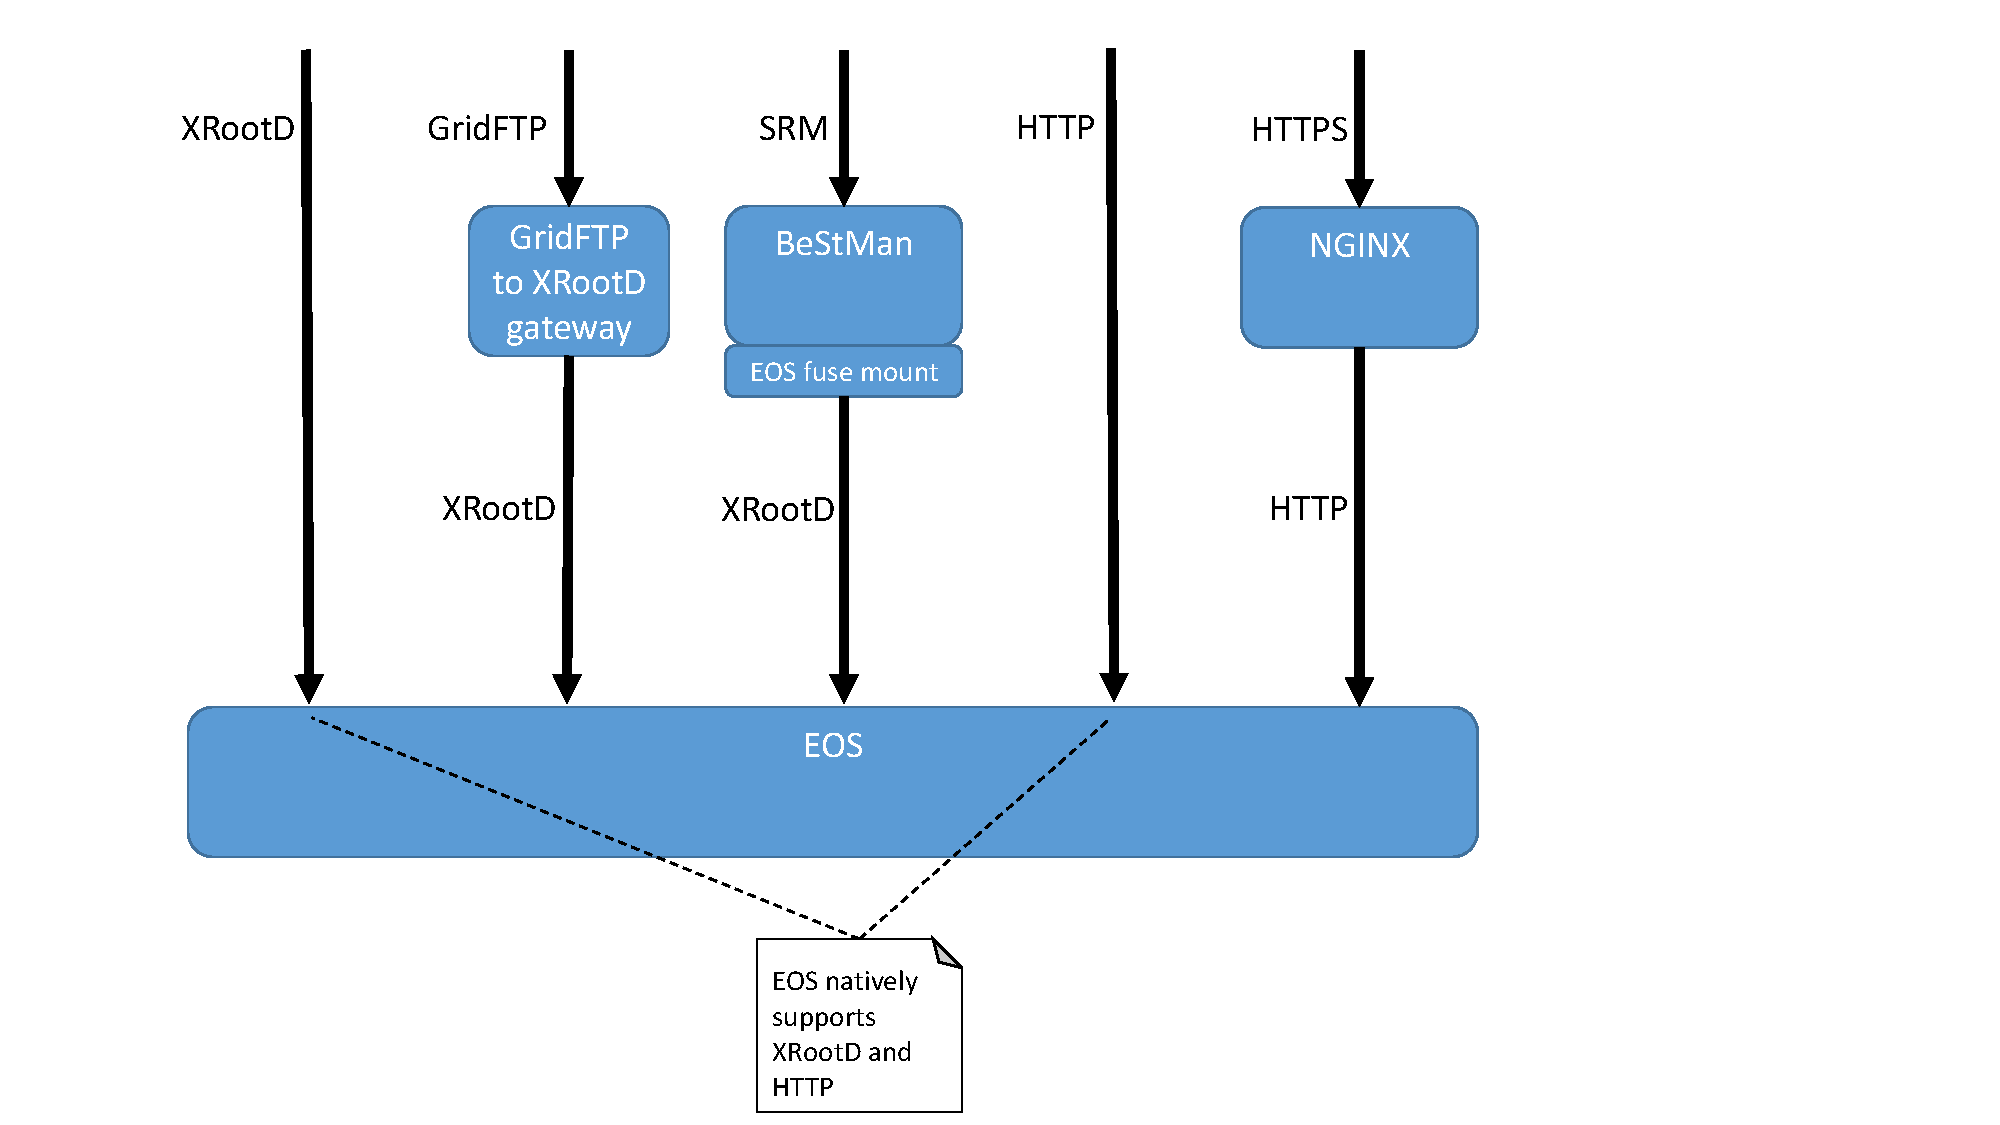
\includegraphics[width=\linewidth]{EOS_supported_protocols}

\newpage
\section{The tape Storage Element}
The tape Storage Element will reconcile the access patterns of users with the access patterns of tape.  Users access patterns are multi-stream, block-oriented and synchronous.  Users start data transfers on demand.  Tape access patterns are single-stream, file-oriented and synchronous. Files are written to and read from tape one file at a time.  Tape transfers are started based on scheduling policies that make efficient use of the underlying tape hardware which is asynchronous in nature.

The following diagram shows the logical components of a tape Storage Element as seen from the outside.  The diagram does not illustrate composition.  For example the disk staging area and the archive namespace may be remote and not owned and contained by a single tape Storage Element.  What is important is how the Storage Element is perceived from the outside.  A user shall be able to connect to the front end of a tape Storage Element and list the files in the archive namespace.  A user shall be able to synchronously copy files into and out of the Storage Element as if they were on disk.

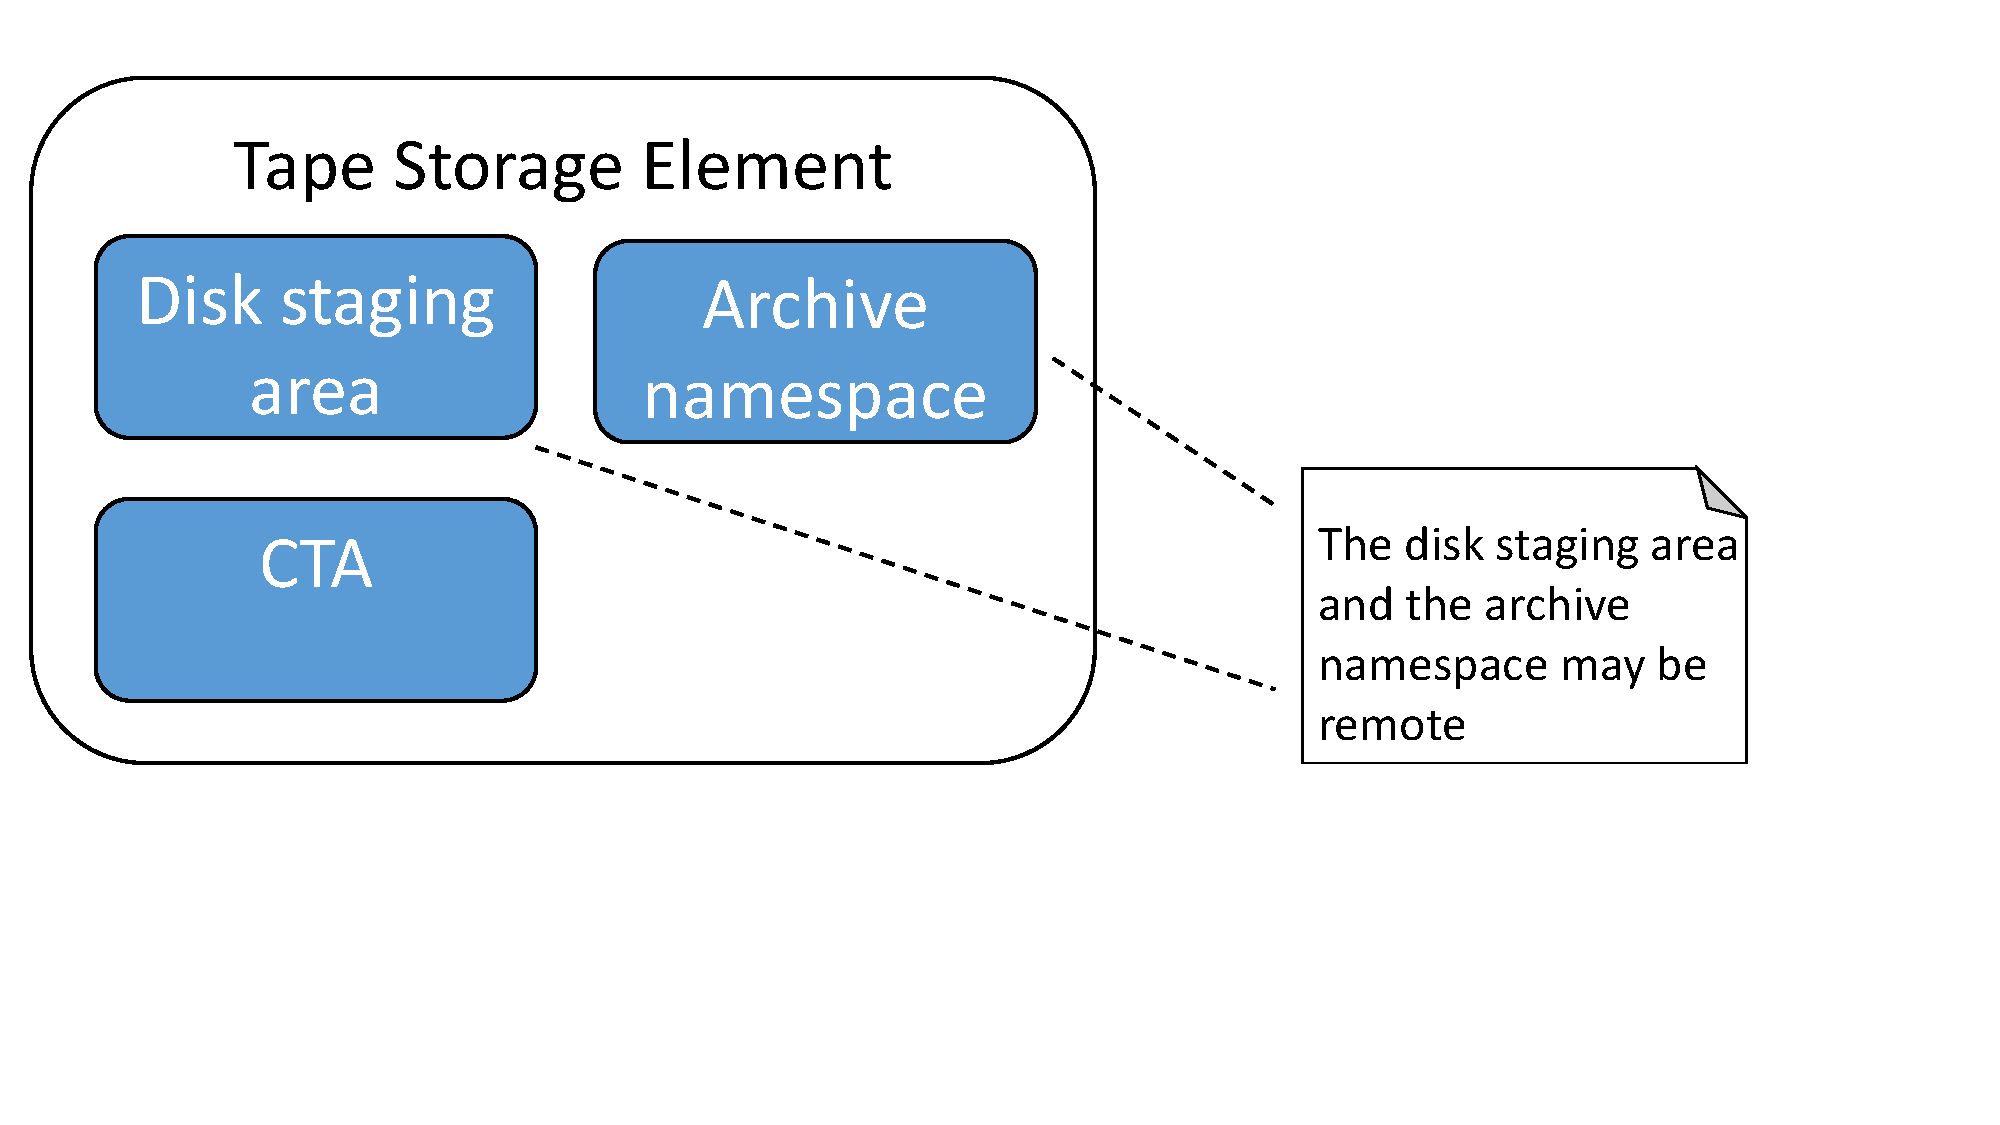
\includegraphics[scale=0.3,trim=0mm 50mm 0mm 0mm]{CTA_tape_storage_element}

As illustrated above, seen from the outside a tape Storage Element shall have its own namespace.  More specifically, for a given file a tape Storage Element shall be able to list the following:
\begin{itemize}
	\item Logical pathname
	\item Authorisation rules
	\item Size
	\item Checksum
	\item Whether or not the file is on disk and/or tape
	\begin{itemize}
		\item On-line: On disk
		\item Near-line: Only on tape and accessible
	\end{itemize}
	\item The tape storage class
\end{itemize}

The availability of a tape file can be classified as on-line, near-line and off-line.  On-line means the file is on disk, near-line means the file is only on tape, off-line means the file is only on tape and that tape is currently not available.  The current CASTOR SRM system permits a user running a \texttt{stat} request to see all three of these classifications.  It is now assumed that end users no longer need to distinguish between near-line and off-line files.  If a file is currently only on tape it shall be reported as near-line even if the tape involved is currently not available.  In the very rare event that a tape becomes unavailable for an extended amount of time because it is being repaired, tape operators will notify the users directly.  There is no need for a tape Storage Element to provide this information to a user via Storage Element commands or APIs.

\newpage
\subsection{How the LHC experiments would use a tape Storage Element}
The following diagram shows the predicted flows of data into and out of a tape Storage Element if it were to be used by one of the LHC experiments.

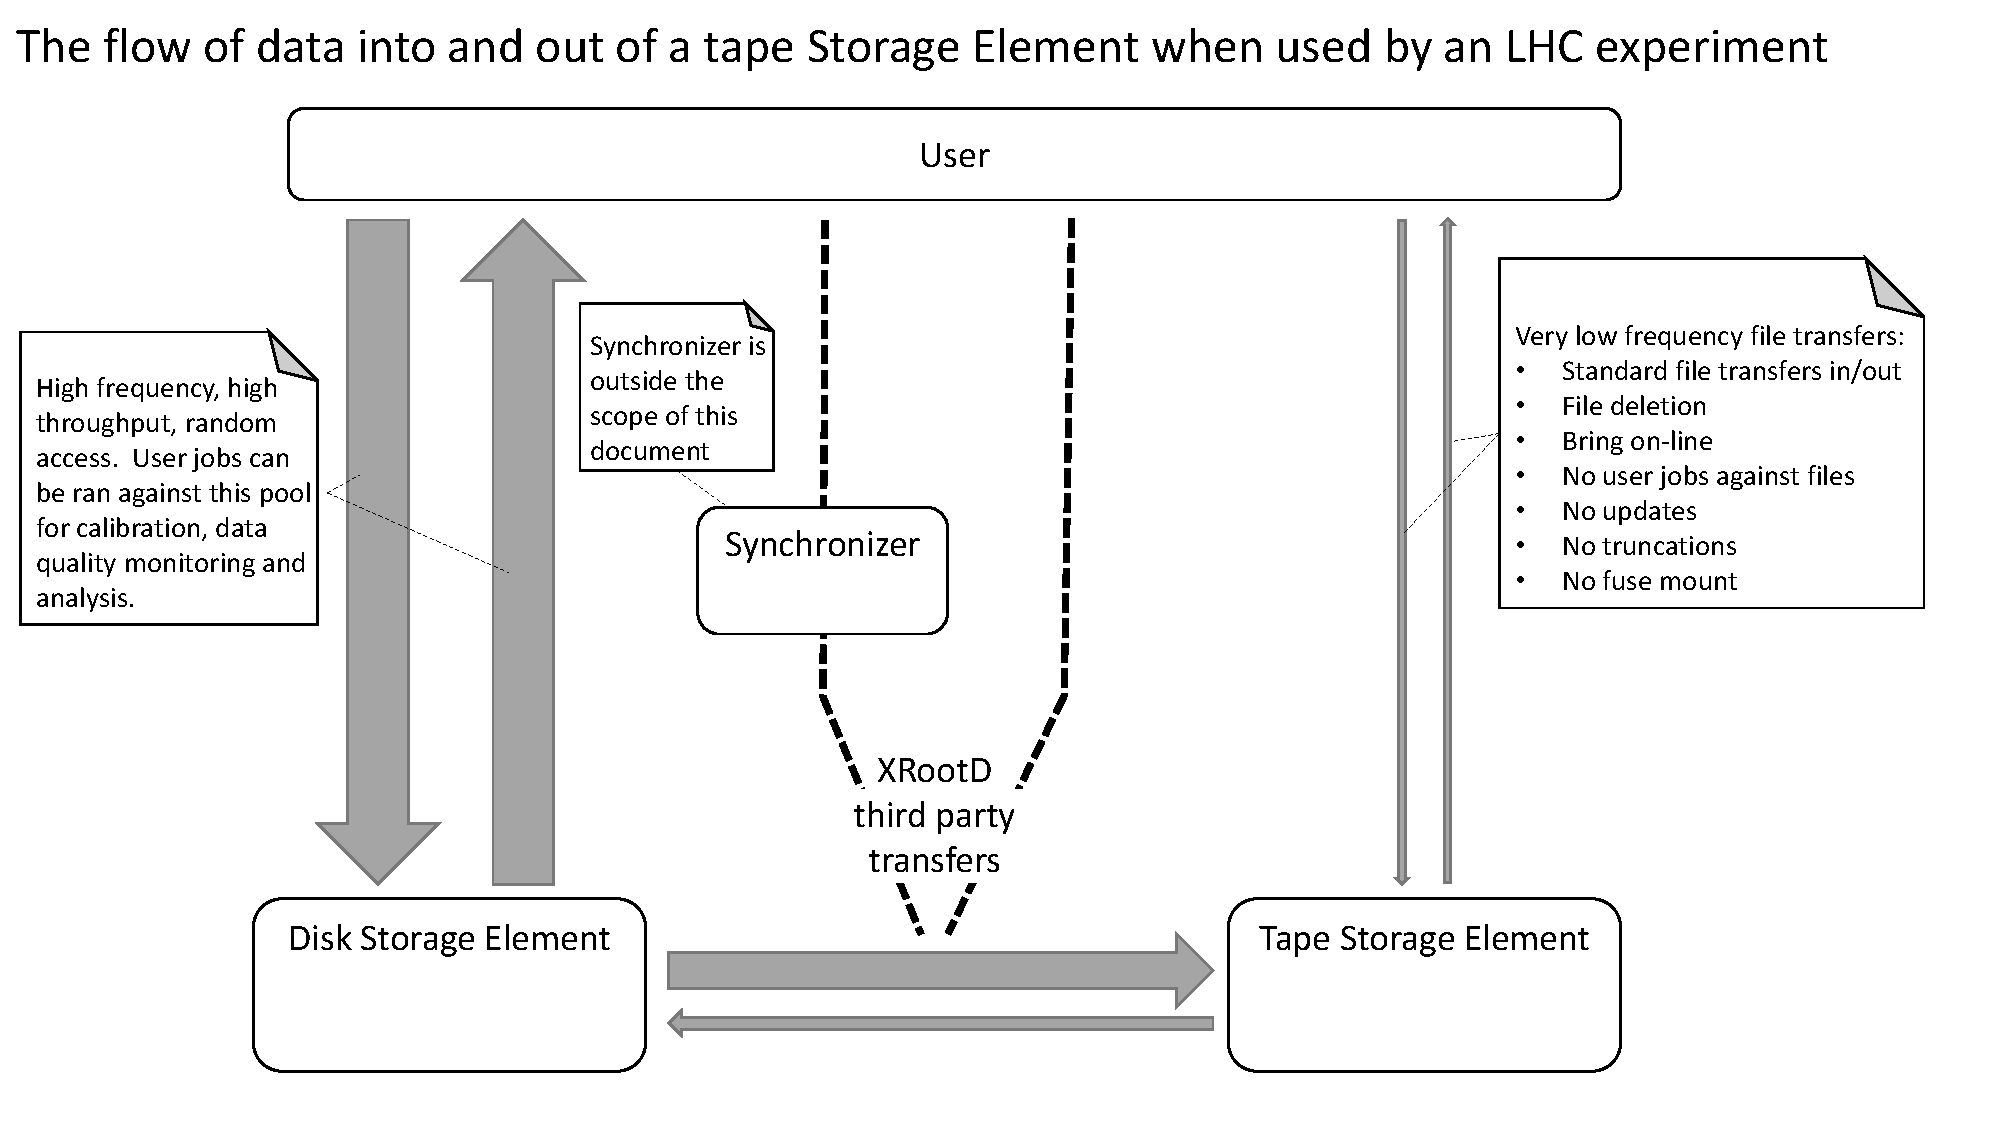
\includegraphics[width=\linewidth]{CTA_tape_se_data_flow_lhc}

An LHC experiment will use a disk Storage Element (a relatively large disk-only EOS instance) as the initial data store for the DAQ data collected from the experiment area.  The same disk Storage Element can also be used by calibration, data quality monitoring and analysis jobs.  An LHC experiment will transfer data from the disk Storage Element to a tape Storage Element by issuing XRootD third party transfer requests.  Some experiments may wish to have an extra synchronizer component that will help automate the bulk transfer of files between the two Storage Elements.  The synchronizer is outside the scope of this document.

\newpage
\subsection{How users of the CERN public CASTOR instance would use a tape Storage Element}
CERN has a public CASTOR instance.  This instance has users who store and access data on behalf of non-LHC experiments and users who require a tape archival system as individuals.

Depending on the ability and willingness of users to adapt the way they access the public CASTOR instance, users could be offered the following migration routes out of CASTOR.  The list is ordered by preference with the most preferable migration route listed first.
\begin{enumerate}
	\item Migrate users to the public EOS instance at CERN.
	\item Migrate users to the public EOS instance at CERN and give them an archiver/synchroniser tool to have their files moved to a hidden public tape Storage Element that cannot be  directly accessed.  The existing EOS archiver is a strong candidate for the archiver/synchroniser tool.
	\item Migrate users to the public EOS instance at CERN and give them access to a public tape Storage Element.
	\item Migrate users to a public tape Storage Element.
\end{enumerate} 

Migration route number 4 is the most undesirable, however in the cases where it is unavoidable the resulting problems can be addressed on a per CASTOR use case.

The 4 major use cases of CASTOR users are as follows:
\begin{enumerate}
  	\item \textbf{Archive once read never}
  	\newline The user simply copies files to CASTOR in order to have them archived to tape.  The files are very rarely, if ever, recalled from tape.
  	\item \textbf{Archive once read many}
  	\newline The user copies files to CASTOR in order to have them archived to tape and to have them available on the CASTOR disk cache for frequent and low-latency read access.
  	\item \textbf{Modify many then archive read never.}
  	\newline The same as the "archive once read never" use case except that the user wishes to initially use CASTOR as a work area to repeatedly modify there files several times before having them marked for archival to tape.
  	\item \textbf{Modify many then archive read many.}
  	\newline The same as the "archive once read many" use case except that the user wishes to initially use CASTOR as a work area to repeatedly modify there files several times before having them marked for archival to tape.
  \end{enumerate}
  Use cases 1 and 2 could be addressed with a simple tape Storage Element that contained an internal disk pool dedicated to being a staging area for tape.  A user archiving a file would synchronously copy that file from their local file system to the staging area.  The file would be asynchronously copied from the staging area to tape at a moment in time that made efficient use of the underlying tape hardware.  Files on the staging area but not yet on tape would be prevented from being deleted.  A user retrieving a file would send a ''bring on-line'' request to the tape Storage Element.  The file would be asynchronously copied from tape to the staging area at a moment in time that made efficient use of the underlying tape hardware.   The user would poll the tape Storage Element for the completion of this asynchronous copy operation.  Once detected the user would synchronously copy the file from the staging area to their local file system.  Any file with a copy on tape would be considered eligible for deletion.  A FIFO or LRU policy would be used to decide which of these eligible file(s) would be deleted next.
  \newpage
  Use cases 3 and 4 would require a more sophisticated Storage Element than use cases 1 and 2.  This sophisticated Storage Element would have to handle files that have three distinct phases in their life cycle as shown in the following diagram:
  
  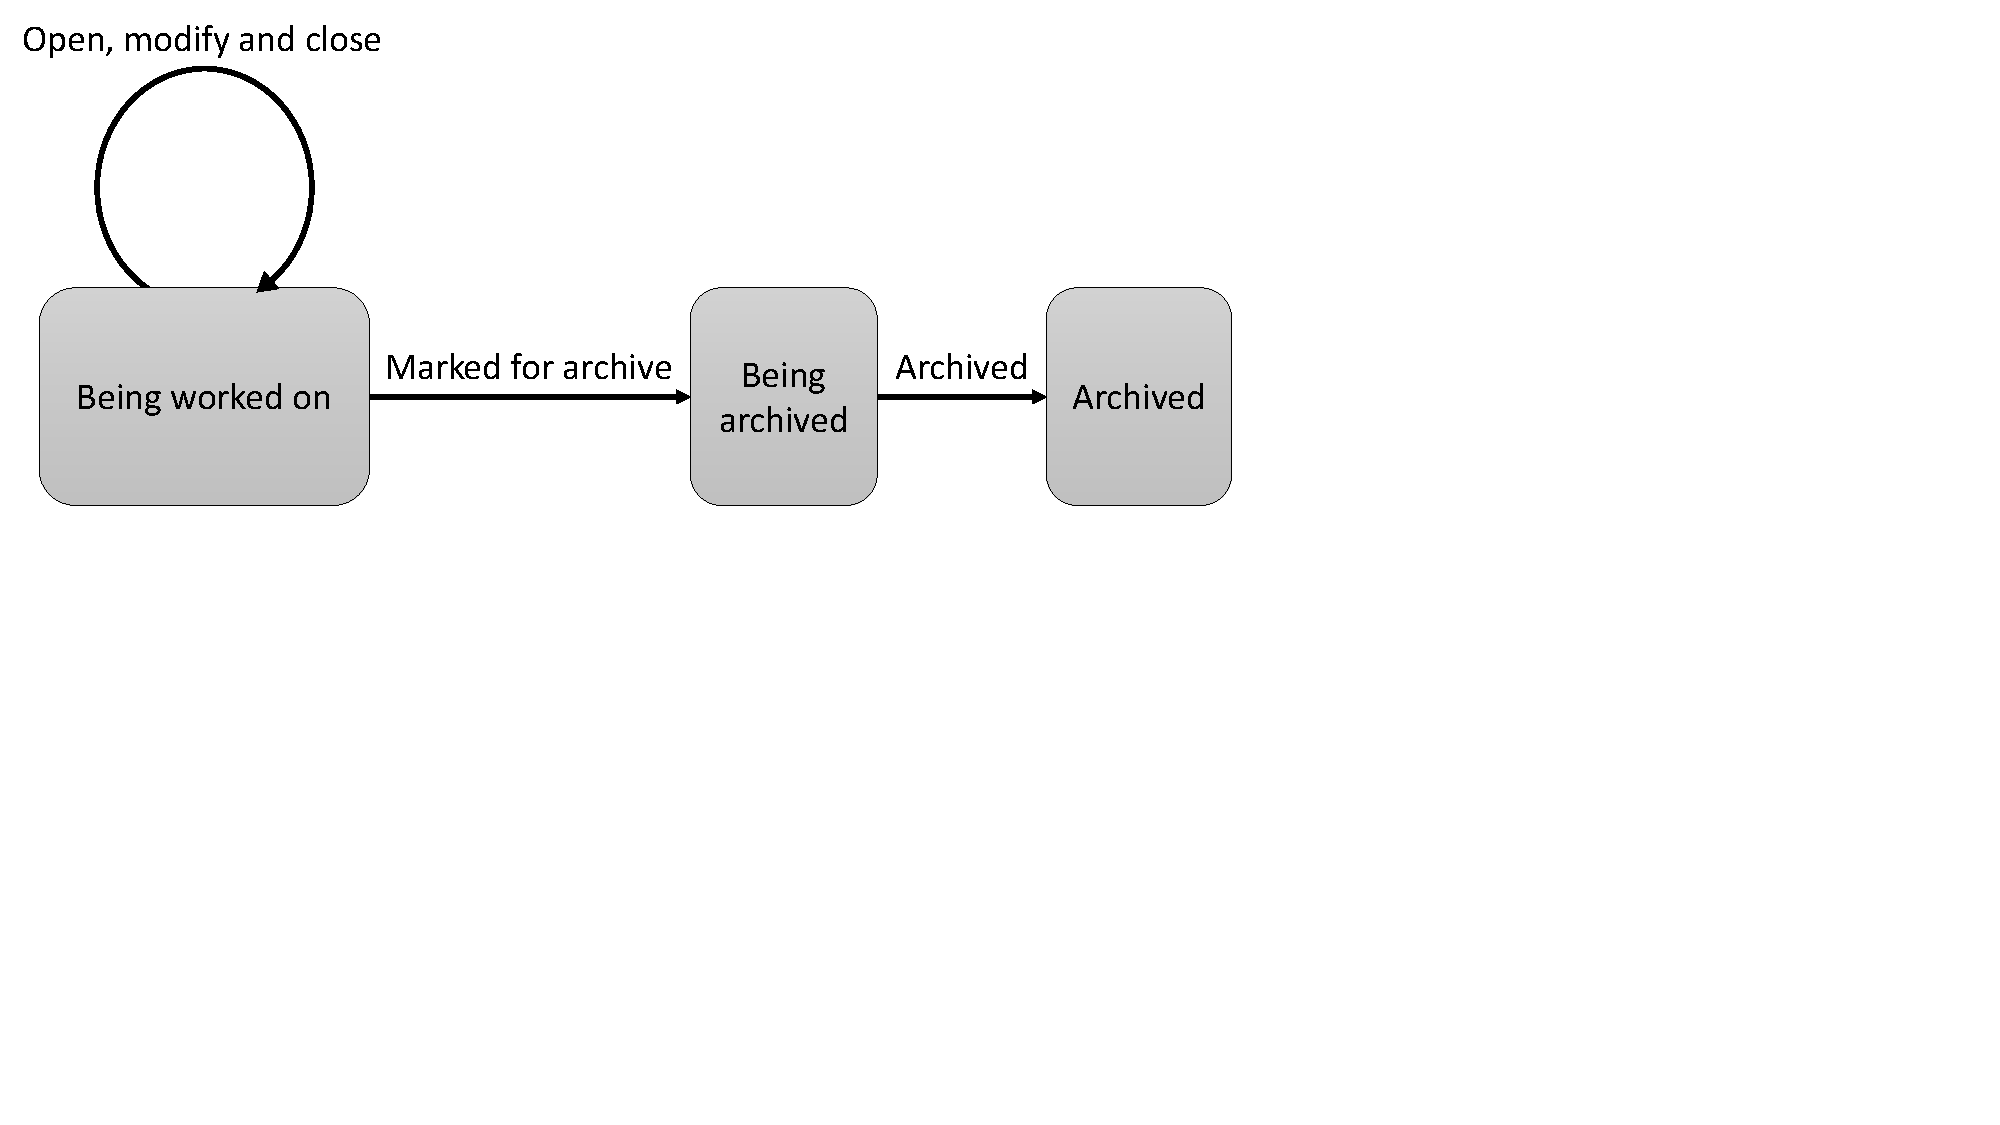
\includegraphics[width=\linewidth,scale=0.8,trim=0mm 100mm 0mm 0mm 0mm]{CTA_3_phase_file}
  
  The Storage Element would have to provide users with one or more commands to allows them to mark files as being complete and ready for archival.  Without such a command the tape Storage Element would risk work in progress files being continuously archived to tape which would needlessly fill tapes with unreferenced previous versions of the files that would result in wasted tape storage space.

  The \texttt{stager\_put} and \texttt{stager\_putdone} command-line tools of CASTOR provide concrete examples of commands that permit users to create files within a single namespace that they can modify many times before having them archived to tape.  The following command-lines give an example scenario:
  \begin{verbatim}
  # Tell CASTOR to a file is going to be opened and modified many times before archival
  stager_put -M /castor/cern.ch/dev/castor_file.txt
  
  # Open the CASTOR file and write the first version
  rfcp my_local_file.txt /castor/cern.ch/dev/castor_file.txt
  
  # Modify a local copy of the file
  vi my_local_file
  
  # Open the CASTOR file for a second time and write the new and final version
  rfcp my_local_file.txt /castor/cern.ch/dev/castor_file.txt
  
  # Tell CASTOR that the file can now be archived to tape
  stager_putdone -M /castor/cern.ch/dev/castor_file.txt
  \end{verbatim}

\newpage
\section{The space management of the disk staging area of a tape Storage Element}

The space management of the disk staging area of a tape Storage Element shall be fully automated.  End users will not be able to delete disk copies from the staging area of a tape Storage Element and leave the associated tape copies untouched.  Users shall only be able to completely delete a file, that is remove its namespace entry along with all of its disk and tape copies.  Tape operators will have administration tools that will allow them to delete disk copies independently of tape copies. 

A tape Storage Element shall use a different space management policy when archiving a file than when retrieving a file.  When a file is being archived the user shall synchronously copy the file into the disk staging area.  The file will stay there until it has been successfully written to tape.  At that moment the file will be deleted from the disk staging area.  When a user retrieves a file that is currently only on tape, the user shall first issue a bring on-line command.  This will result in the tape system asynchronously copying the file from tape to disk.  The user shall poll the tape Storage Element to detect when the file is on disk.  Once this has happened and the user has detected it, the user will synchronously copy the file out of the disk staging area.  The file shall remain in the disk staging area until it is garbage collected using an appropriate strategy, for example LRU or FIFO.

\newpage
\section{Two design proposals for a tape Storage Element}

The are currently two design proposals for a tape Storage Element.

\begin{itemize}
	\item EOSTAPE
	\begin{itemize}
		\item Put CTA behind EOS.
	\end{itemize}
	\item Orchestrator
	\begin{itemize}
		\item A staging manager that uses EOS as a staging area for CTA.
	\end{itemize}
\end{itemize}

There are two main differences between the proposals.
\begin{itemize}
	\item The control path from the user to EOS and CTA
	\item Where the archive namespace will be stored
\end{itemize}

The following diagram illustrates the different user control paths of EOSTAPE and the orchestrator.

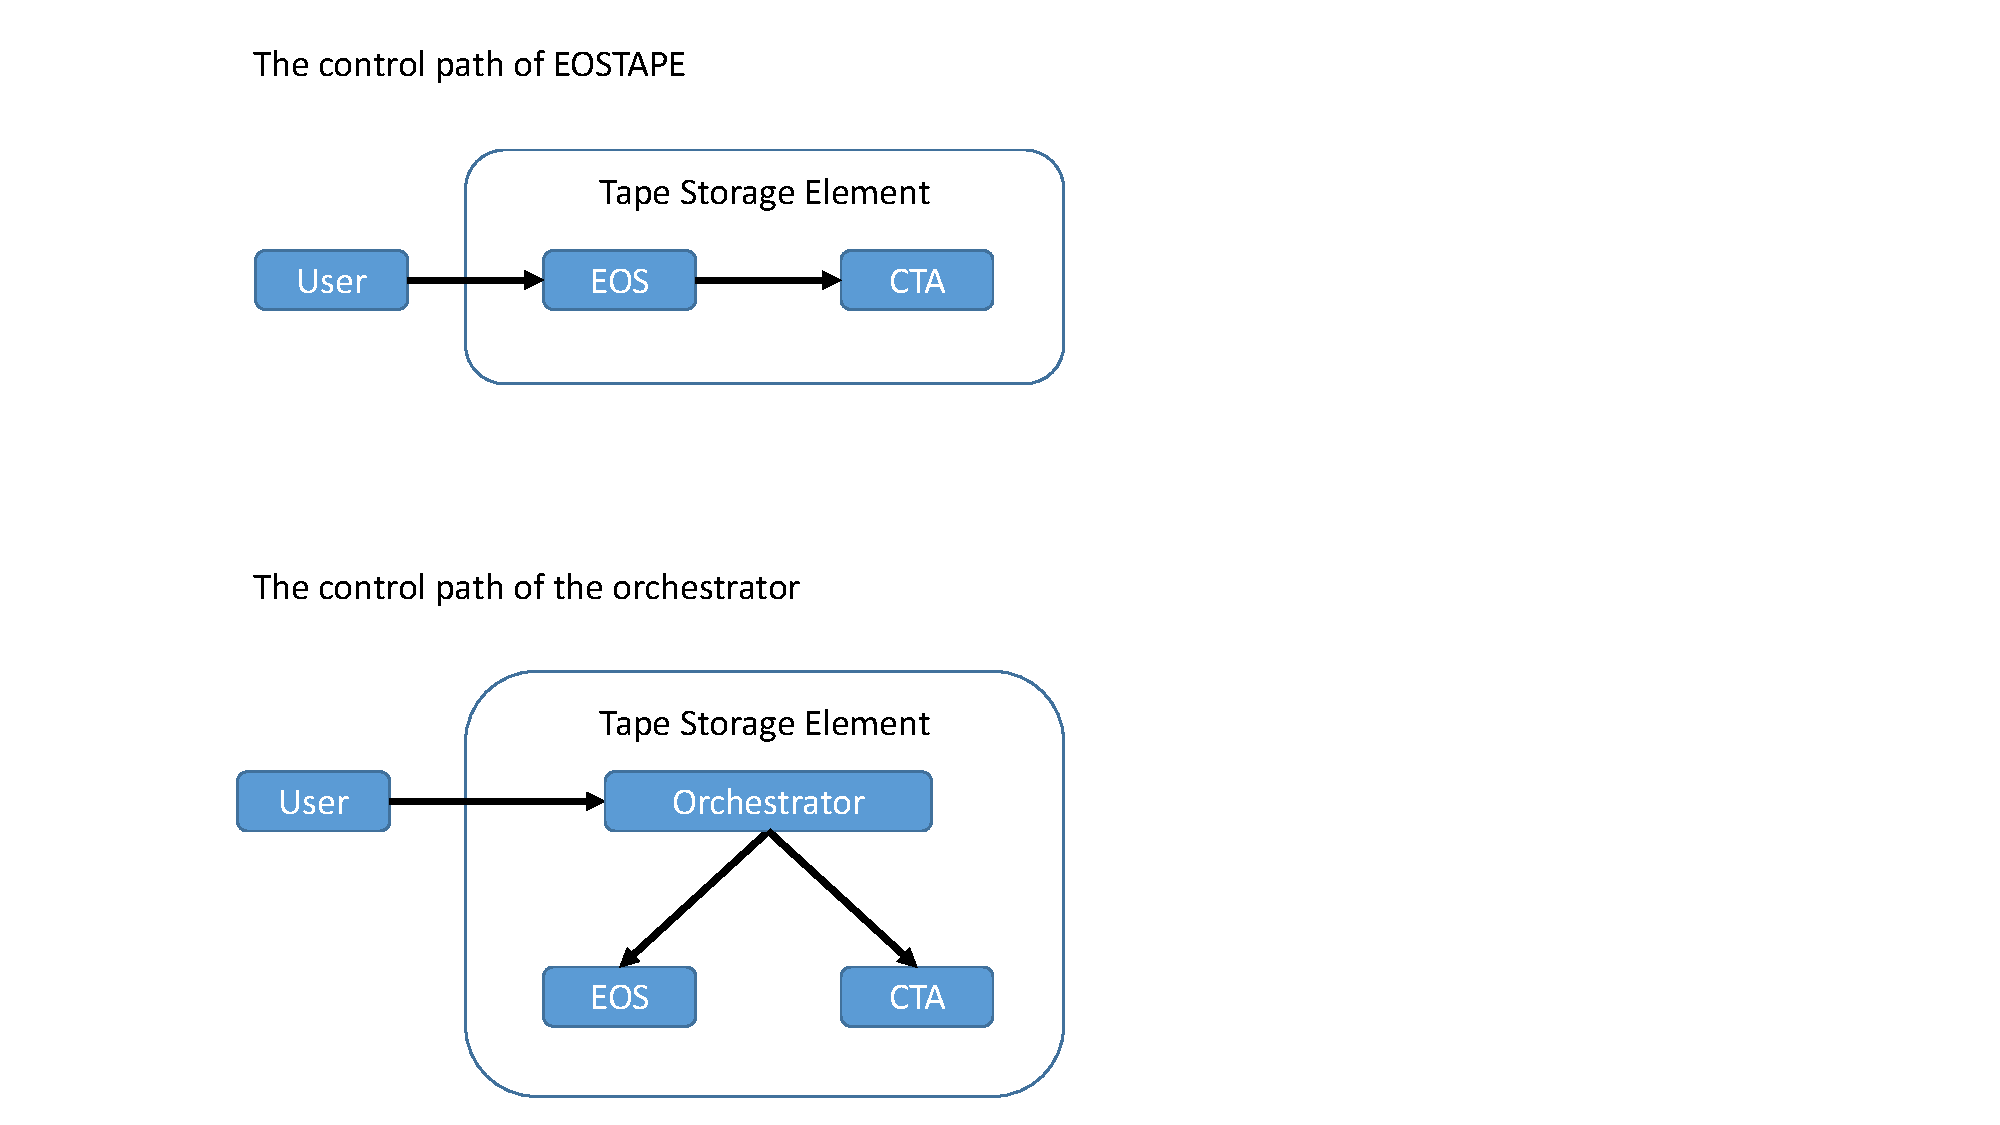
\includegraphics[width=\linewidth]{EOSTAPE_orchestrator_control_paths}

The control path of EOSTAPE is from the user to EOS to CTA.  The control path of the orchestrator is from the user to the orchestrator and then down to EOS and CTA.  In other words with EOSTAPE the internal EOS instance implements the equivalent of the orchestrator.  It should be noted that the EOSTAPE solution would not require EOS to be tailored or modified specifically to handle tape.  An EOS workflow engine is currently under development.  It will be possible to configure this workflow engine to act as an orchestrator.  The front end of CTA is an XRootD server.  The workflow engine will communicate with the CTA front end by either sending parametrised XRootD requests or by executing external CTA specific scripts.

\newpage
The following two diagrams illustrate the difference between EOSTAPE and the orchestrator with respect to where the archive namespace shall be stored.

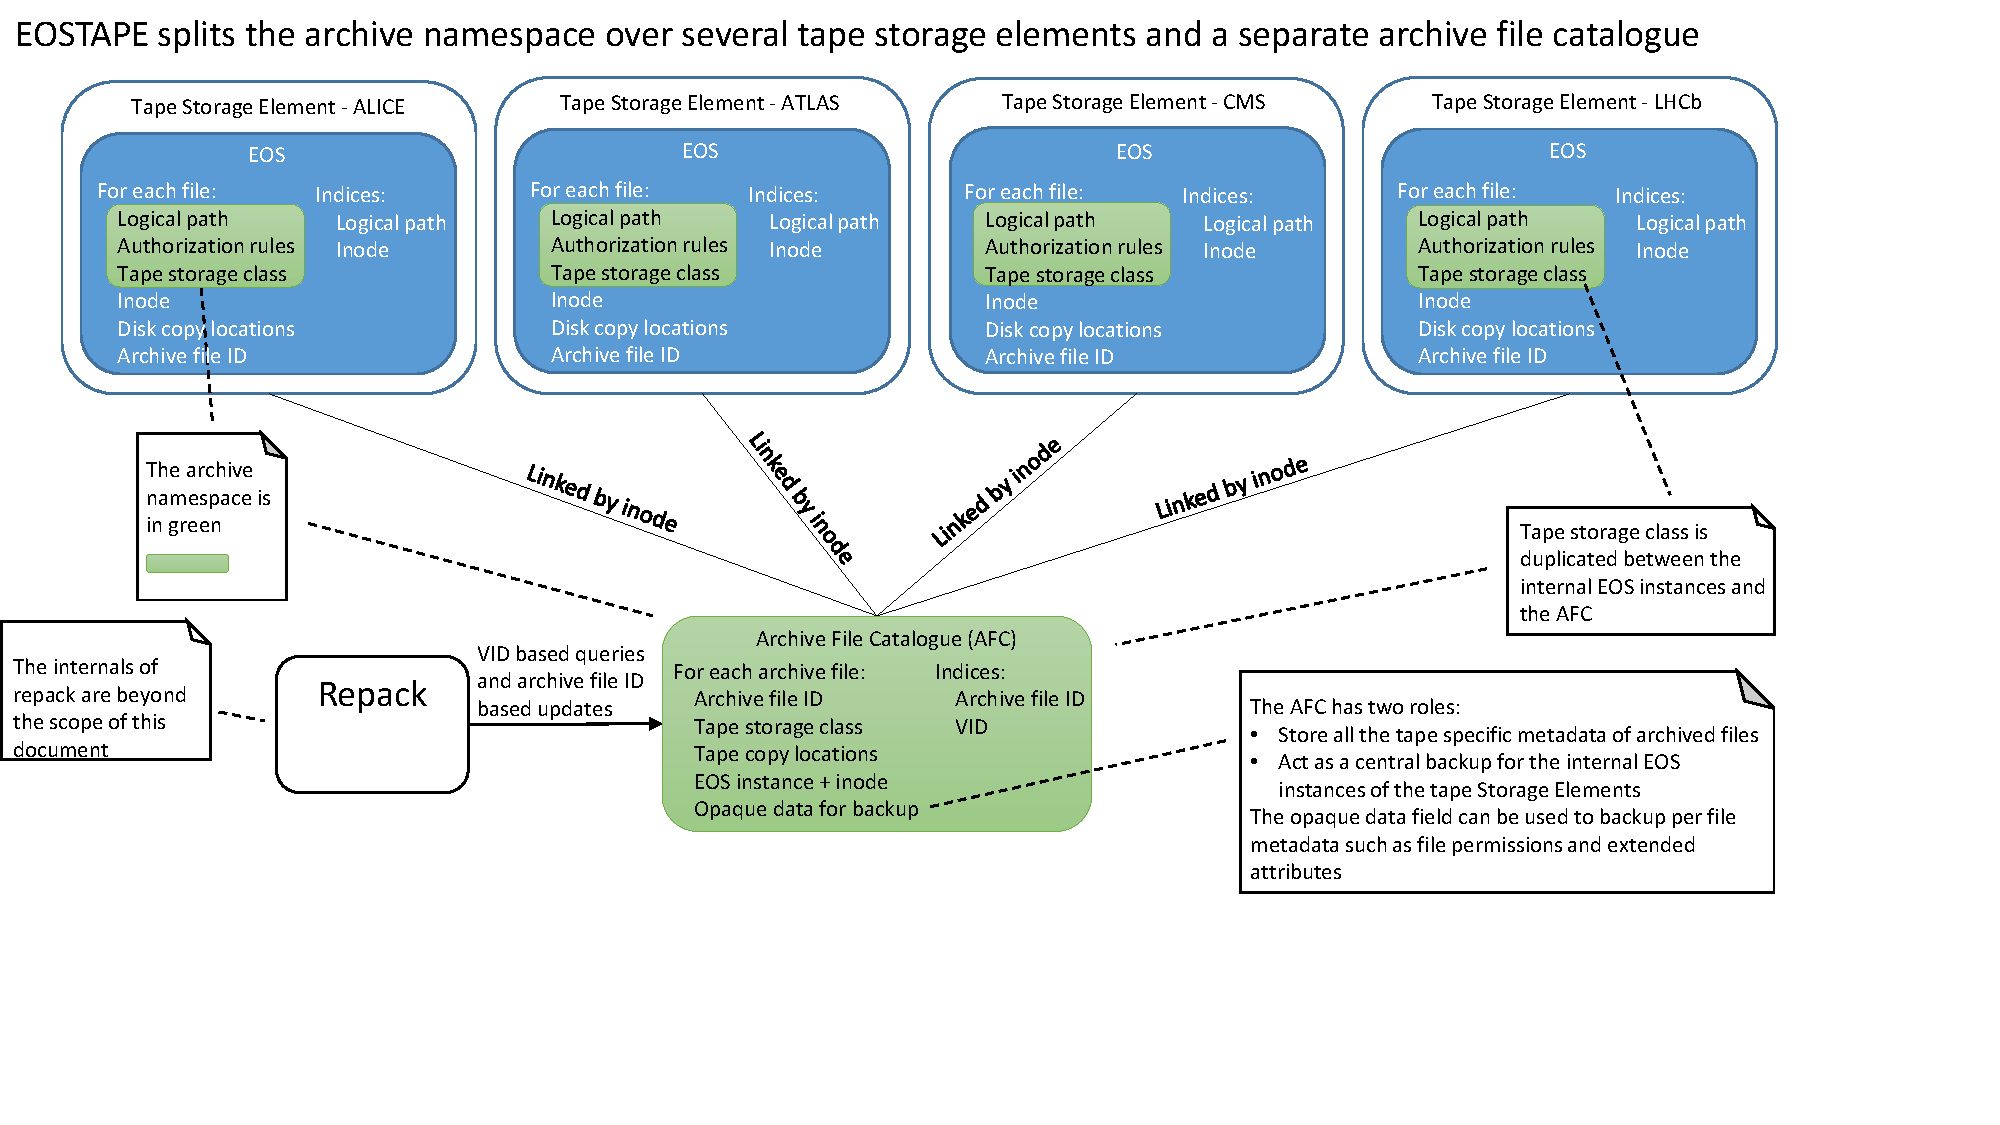
\includegraphics[width=\linewidth, trim=0mm 40mm 35mm 0mm]{EOSTAPE_namespaces}

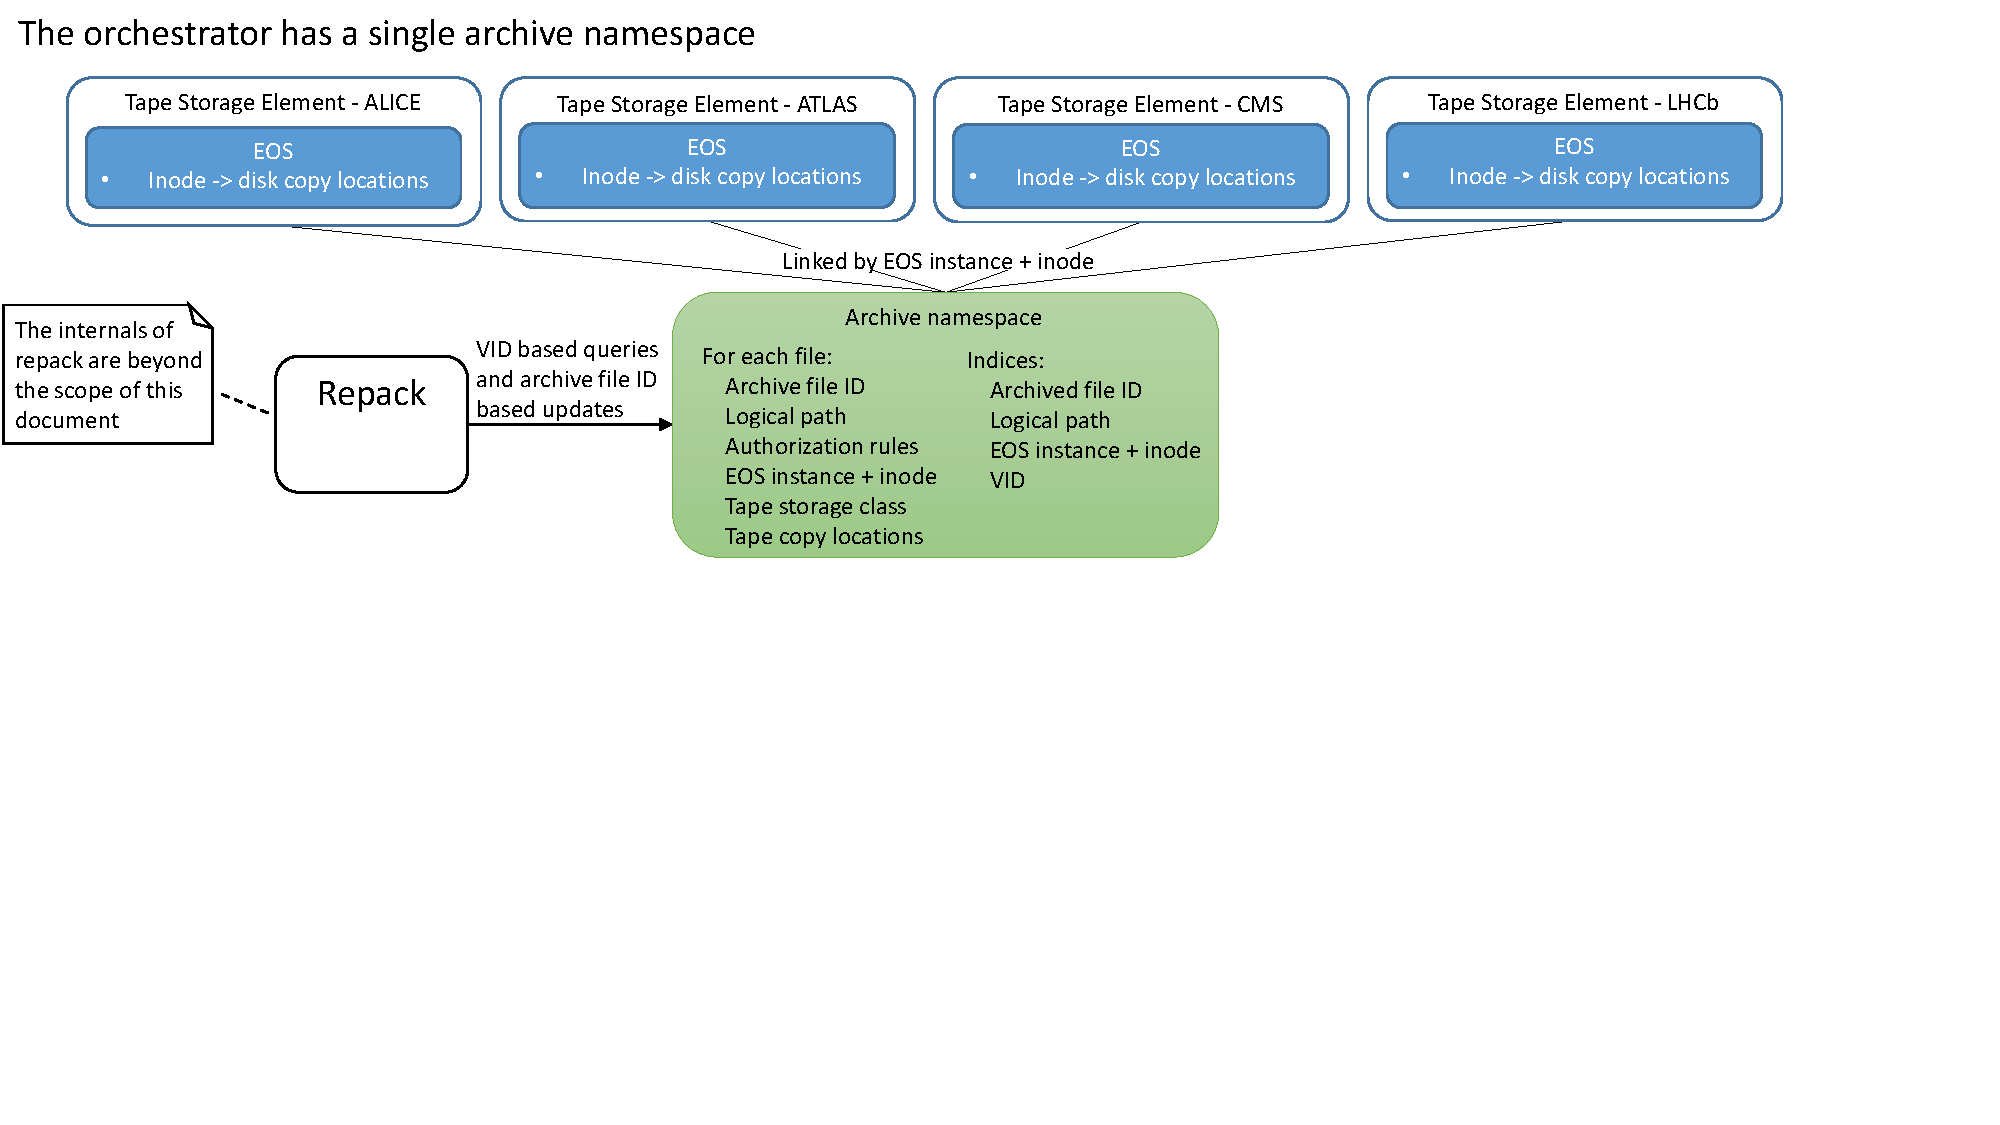
\includegraphics[width=\linewidth, trim=0mm 90mm 35mm 0mm]{Orchestrator_namespaces}

The archive namespace of EOSTAPE is divided up over one or more EOS instances and a single Archive File Catalogue (AFC).  The orchestrator has a single archive name server.

EOSTAPE has an AFC in order to provide a central, efficiently indexed catalogue for repack operations.  A large repack campaign would be carried out by a dedicated repack instance that would rely on the AFC.  The tape Storage Elements of experiments should be isolated from this repack instance, it should not need to communicate with them in order to do its job.

The internal EOS instances of EOSTAPE shall not know about individual tape copies.  This information shall be private to the AFC.  The internal EOS instances shall not even know the current number of existing tape copies for a given file.  They will of course know the tape storage class of a given file which will give a good indication as to how many tape copies there should be.  They will also know if a file is safely stored on tape.  There will not be any EOS commands that users will be able to use to query EOS for information about individual tape copies.  The internal EOS instance will be notified by CTA when a file is safely stored on tape.  The decision of how many copies need to be written to tape for a file to be deemed safely stored on tape is a decision to be taken by CTA.

\newpage
\section{EOSTAPE}
The following diagram shows a very high level view of the architecture of EOSTAPE by providing an example of how a file would be archived to tape.

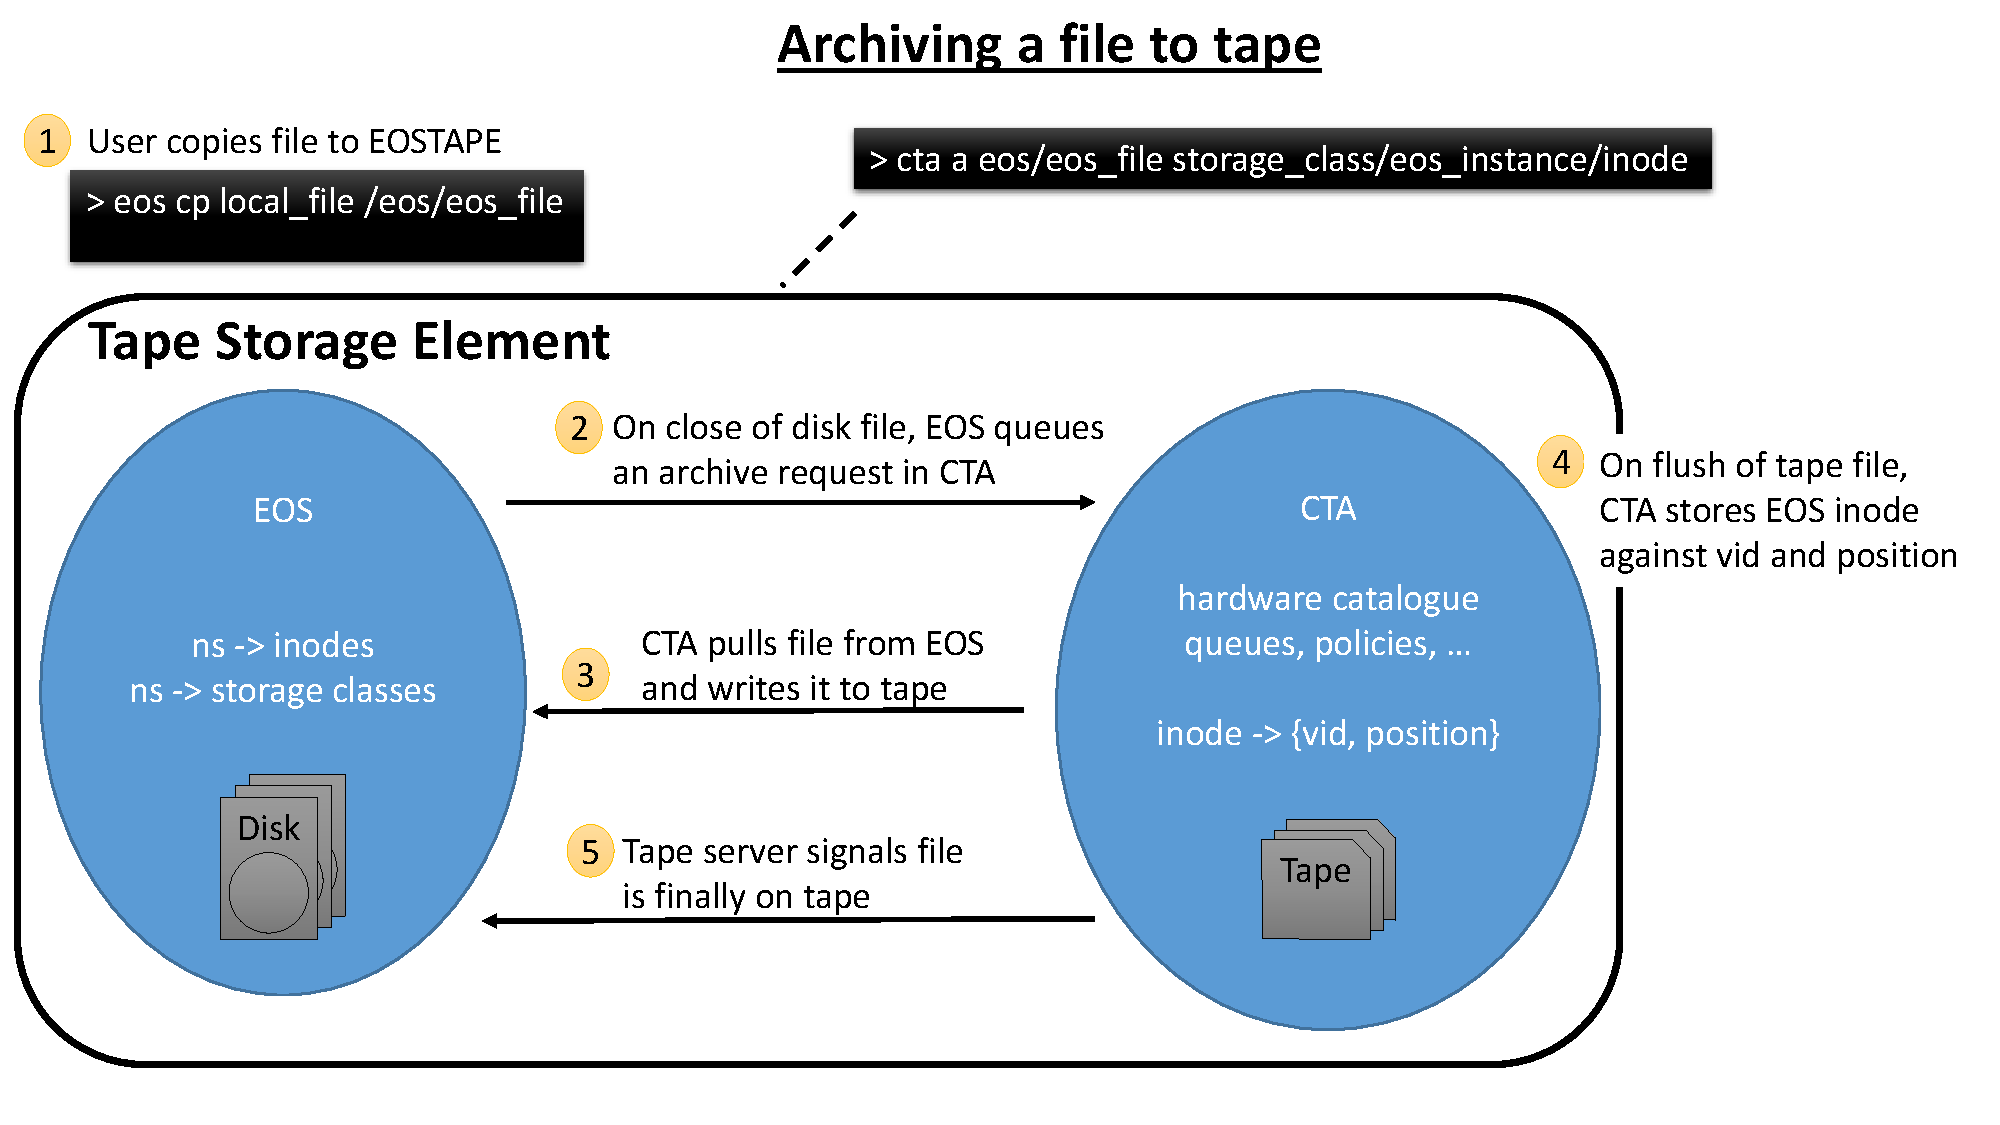
\includegraphics[width=\linewidth]{EOSTAPE_high_level_archive}

The following diagram increases the level of detail.

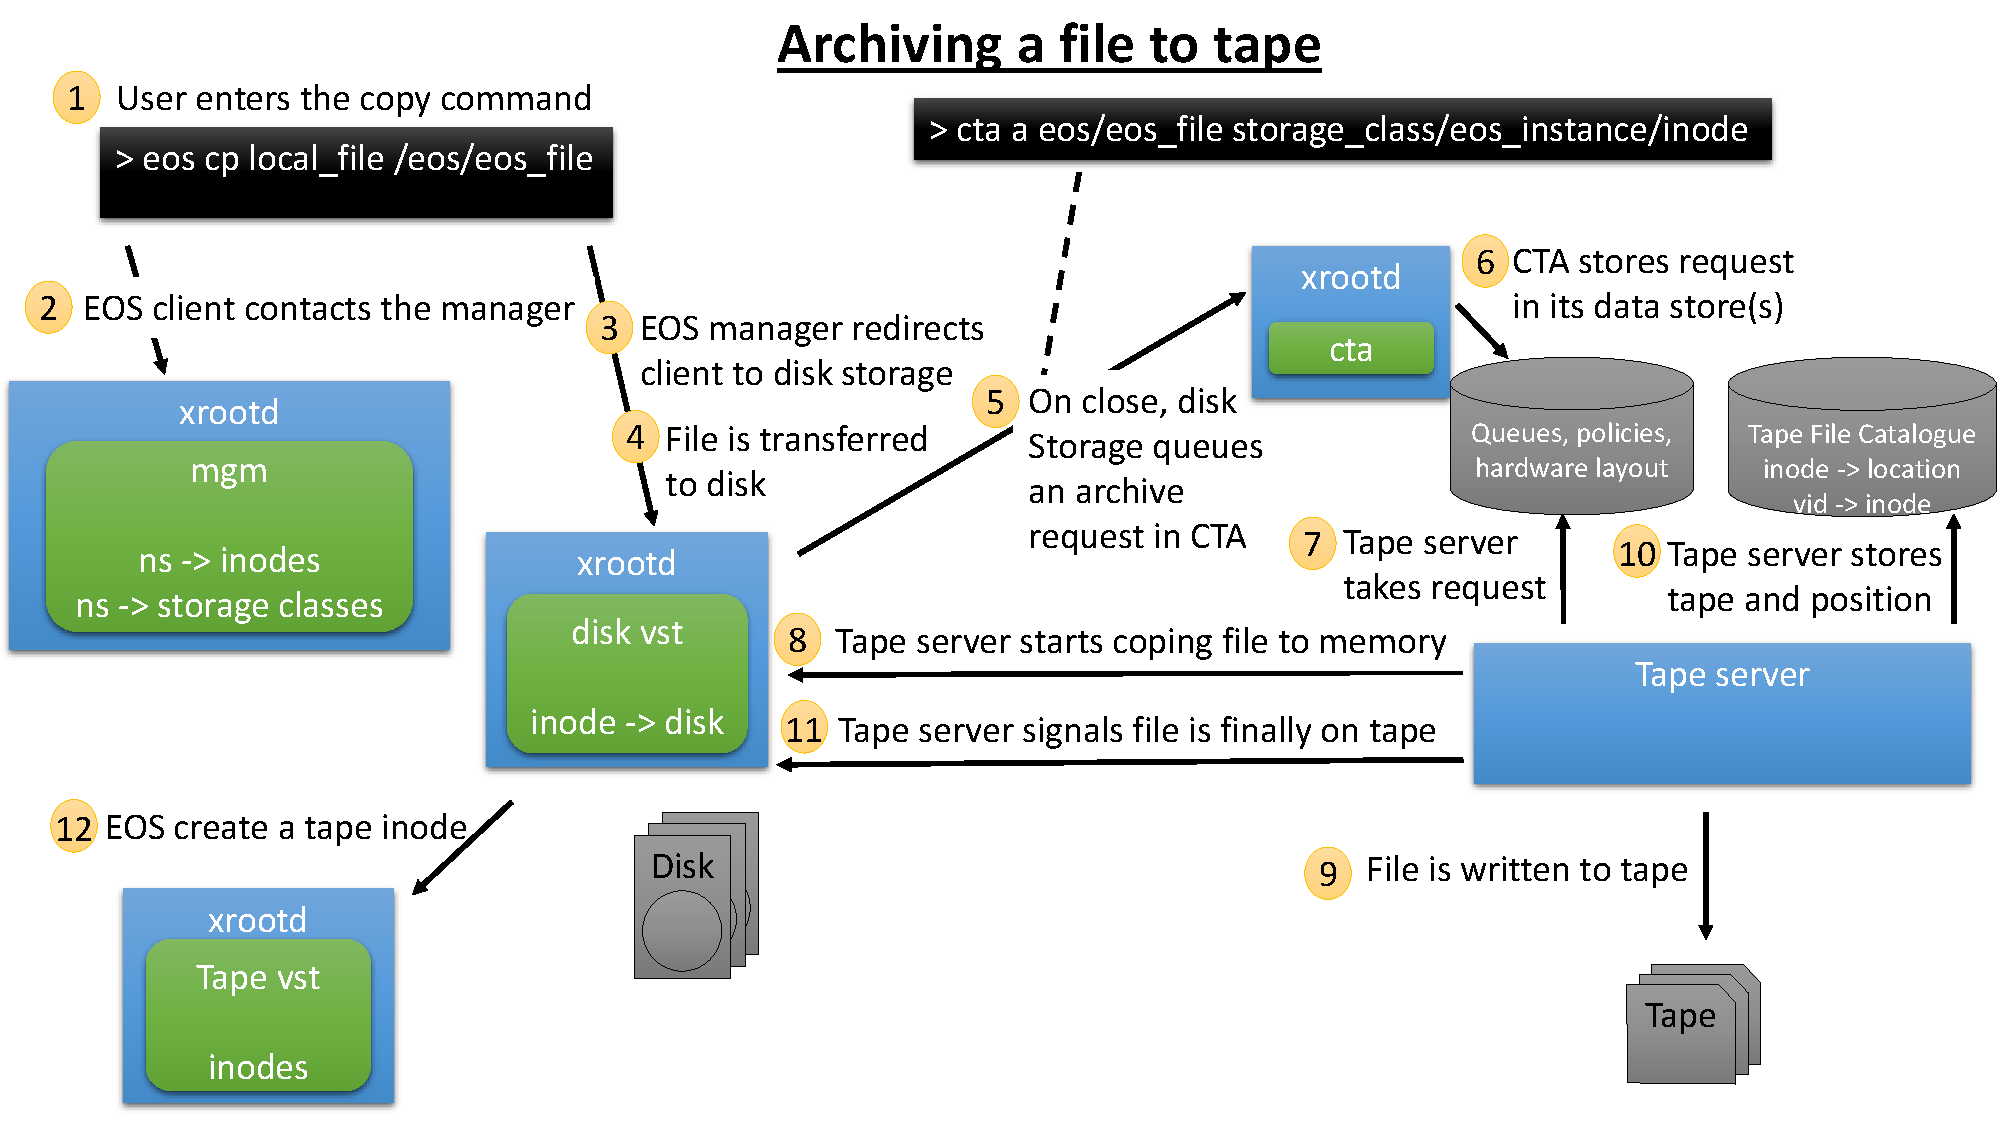
\includegraphics[width=\linewidth]{EOSTAPE_simple_archive}

\newpage
\subsection{Archive a file}
The following list of steps increases the level of detail again for the use case of archiving a file to tape.  The level of detail used in this list should be sufficient to answer any questions about the technical feasibility of EOSTAPE. 
\begin{enumerate}
\item User creates a directory within the EOS namespace for files that are to be archived to tape.

\texttt{eos mkdir /eos/tape\_dir}

\item The user associates the appropriate layouts and workflow with the directory.

\begin{verbatim}
	# Disk files should start out as having 2 replicas
	eos attr set default=replica /eos/tape\_dir

	# The policy to migrate files and keep them in the disk pool

	# If a default policy is used and a file is written, we call a parameterised URL
	eos attr set sys.workflow.default="onclosew:*/*:call:http://cta.cern.ch?<params>" /eos/tape\_dir

	# If the migration policy is used by the cta user and a file was read with a successful close,
	# we register it in the tape location(space) and drop it from the default locations
	attr set sys.workflow.migrate="oncloser:cta/cta:register:tape,oncloser:cta/cta:drop:default"
	    /eos/tape\_dir

	# If a file was written by the cta user and the recall policy was used,
	# nothing has to be done - one can just omit that!
	attr set sys.workflow.recall="onclosew:cta/cta:none" /eos/tape

	# Add a condition on the LRU policies that files cannot be garbage
	# collected if they don't have a location in the tape space

	SYNTAX TO BE DECIDED
\end{verbatim}
\item The user associates the destination tape storage class with the directory by setting an extended attribute.

\texttt{eos attr set tape\_storage\_class=daq\_raw\_2\_copies}

\item The user runs a command-line tool to synchronously copy a file into the internal disk staging area of EOSTAPE with no overwrite:

\texttt{eos cp -k local\_file /eos/murrayc3/tape\_dir/tape\_file}

\item The command-line tool connects to the XRootD server with the MGM plug-in and requests the destination file \texttt{tape\_file} be opened for writing.

\item The MGM plug-in asserts the destination file does not already exist.

\item The MGM plug-in redirects the client to a disk FST.

\item The client writes the data and closes the file on the disk FST

\item The disk FST notifies the MGM of the close for write.

\newpage
\item The MGM plug-in executes the appropriate workflow and connects to the CTA XRootD front-end and queues a request to archive the file.  The request includes:
\begin{itemize}
	\item EOS instance name
	\item EOS inode
	\item File size
	\item File checksum
	\item Destination tape storage class
\end{itemize}

\item The CTA XRootD front-end stores the archive request in the CTA object store.

\item A tape server pulls the need to mount a tape from the CTA object store and does so.

\item The tape server pulls the archive request from the CTA object store.

\item The tape server connects to the XRootD server with the MGM plug-in and requests the source disk file based on inode be opened for reading.

\item The MGM redirects the tape server to the disk FST.

\item The tape server opens the file on the disk FST for reading.

\item The tape server reads blocks from the file on the disk FST and writes them to the tape.

\item The tape server closes the file on the disk FST.

\item After enough files have been written to tape, the tape server synchronously flushes the tape drive cache in order to guarantee that all of the files since the previous flush are now safely on tape.

\item The tape drive notifies the MGM that the file is safely on tape by sending the EOS inode of the file \texttt{00b81351} together with the \texttt{migrated} workflow event.

\texttt{xrdfs eostape "/?eos.lfn=fxid:00b81351\&eos.workflow=migrated"}

\item The MGM marks the file as being on tape.

EOS currently has a queue in the MGM for file conversions.  A second queue to run workflows can be added. Workflows would stay in the queue until they are successful or a retry policy expires them. This boils down to moving virtual files between directories representing a state.  An operator could manually re-trigger things by just moving a virtual file back into a queue. Supporting workflows in  this way will be trivial due to the fact that every low-level command is already implemented today in order to provide the current EOS support for ''conversions/converters''.

\end{enumerate}

The EOS workflow engine is not only something useful for coordinating access to tape. It could be useful to have completed transfers from the experiment areas at CERN trigger the delayed creation of replicas in WIGNER. The CERNBOX backup procedure could also be specified and implemented using an EOS workflow. There are many applications for EOS workflows outside of integrating CTA.

\newpage
\subsection{Retrieve a file}
The following list of steps explain how EOSTAPE can be used to retrieve a file from tape.  The level of detail used in this list should be sufficient to answer any questions about the technical feasibility of EOSTAPE. 

\begin{enumerate}
\item The user runs a command-line tool to synchronously copy a file from the internal disk staging area of EOSTAPE to their local disk.

\texttt{eos cp /eos/murrayc3/tape\_dir/tape\_file local\_file}

\item The command-line tool connects to the XRootD server with the MGM plug-in and requests the destination file \texttt{tape\_file} be opened for reading.

\item The MGM plug-in asserts the file is near-line.  The file is accessible on tape but is not a disk.  The MGM plug-in therefore sends the command-line tool an error message such as ''\texttt{File X is not on disk, please bring it on-line}''.

\item The user runs a command-line tool to request the file be prepared for access and therefore staged to disk.

\texttt{xrdfs prepare -s root://eostape//eos/murrayc3/tape\_dir/tape\_file}

The XRootD prepare command is currently ignored by EOS.  Interpreting this command would be part of the future workflow support of EOS.

\item The MGM plug-in checks the file is not already on disk, that the file is on tape and that there is currently no ongoing prepare operation for the file.

It is the responsibility of EOS to not create a CTA retrieval request if a file is already on disk.  It is however the responsibility of CTA to collapse multiple queued requests for the same retrieval operation.

\item The MGM plug-in connects to the CTA XRootD front-end and queues a request to retrieve the file from tape.  The request includes:
\begin{itemize}
	\item EOS instance name
	\item EOS inode
	\item File size
	\item File checksum
\end{itemize}

\item The CTA front end checks that CTA knows the tape file location based on the EOS instance and EOS inode.

\item The CTA front end stores the retrieval request in the CTA object store.

\item In the meantime the user runs a command-line tool in a loop to decide when the file has been staged to disk.

\texttt{eos fileinfo /eos/murrayc3/tape\_dir/tape\_file}

\item A tape server pulls the need to mount a tape from the CTA object store and does so.

\item The tape server pulls the retrieval request from the CTA object store.

\item The tape server connects to the XRootD server with the MGM plug-in and requests the destination disk FST file be opened for writing based on its inode.

\item The MGM plug-in redirects the tape server to a disk FST.

\item The tape server opens the file on the disk FST for writing.

\item The tape drive reads blocks from the tape and writes them to the disk FST file.

\item The tape drive closes the disk FST file.

\item The disk FST notifies the MGM that the file has been staged to disk.

\item The user notices the file is now on disk and in response runs a command-line tool to synchronously copy the file from internal disk staging area of EOSTAPE to their local disk.

\texttt{eos cp /eos/murrayc3/tape\_dir/tape\_file local\_file}

\item The command-line tool connects to the XRootD server with the MGM plug-in running and requests the destination file tape\_file be opened for reading.

\item The MGM plug-in asserts the file exists on disk and redirects the command-line tool to the disk FST.

\item The command-line tool opens, reads and closes the file on the disk FST.
\end{enumerate}

\subsection{List files to see which are on-line and which are near-line}

The only command-line tool that can currently shows whether or not a file is on tape is \texttt{eos} ran with its \texttt{fileinfo} command.  Here is an example of running \texttt{eos} against a single file:

\texttt{eos fileinfo pathname}

If the file was on tape then there would be a corresponding line with the value of the \texttt{schedgroup} column set to \texttt{tape}.  The user would only know the file was safely on tape.  They would not know about the individual tape copies.

Like other \texttt{eos} commands, \texttt{fileinfo} can be piped over \texttt{stdin} as opposed to being supplied on the command-line.  The following example shows how to use this technique to display information about a list of files with a single invocation of the \texttt{eos} command:

\texttt{cat files.txt}\newline
\texttt{pathname1}\newline
\texttt{pathname2}\newline
\texttt{pathname3}\newline
\texttt{...}\newline
\texttt{cat files.txt | awk '\{print "fileinfo " \$0\}' | eos}

The \texttt{fileinfo} command does not provide any support for filename expansion.  The \texttt{eos ls} and \texttt{find} commands provide for filename expansion but their output does not include any space information.  In other words their output does not tell the user whether or not a file is on tape.  If users will require filename expansion when displaying which files are on tape then the \texttt{eos} command-line tool and its associated server side code will need to be modified accordingly.  User would then be able to type commands like the following:

\texttt{eos find -{}-fileinfo directory\_path}

\texttt{eos ls -l directory\_path}

\subsection{Remove a file}

An end user of EOS will only be able to delete a file completely.  They will not be able to delete just the disk copy of a file and leave the tape copy intact.  The command the user will use is as follows:

\texttt{eos rm pathname}

Contrary to an end user, a tape operator will be able to delete just the disk copy of a file.  To do this they will use the following command.

\texttt{eos file drop pathname file\_system\_id}

\subsection{How EOSTAPE could be used directly by existing users of the CERN public CASTOR instance}

There are 4 proposed migration routes out of CASTOR for current users of the CERN public CASTOR instance.  The fourth and most undesirable migration route is the one to one replacement of CASTOR with EOSTAPE.  If this migration route cannot be avoided, then there are two proposals as to how EOSTAPE would support this migration route:
\begin{itemize}
	\item Deploy an EOSTAPE Storage Element with two internal EOS disk pools: a work pool for repeatedly opening and modifying files and a staging pool for tape.
	
	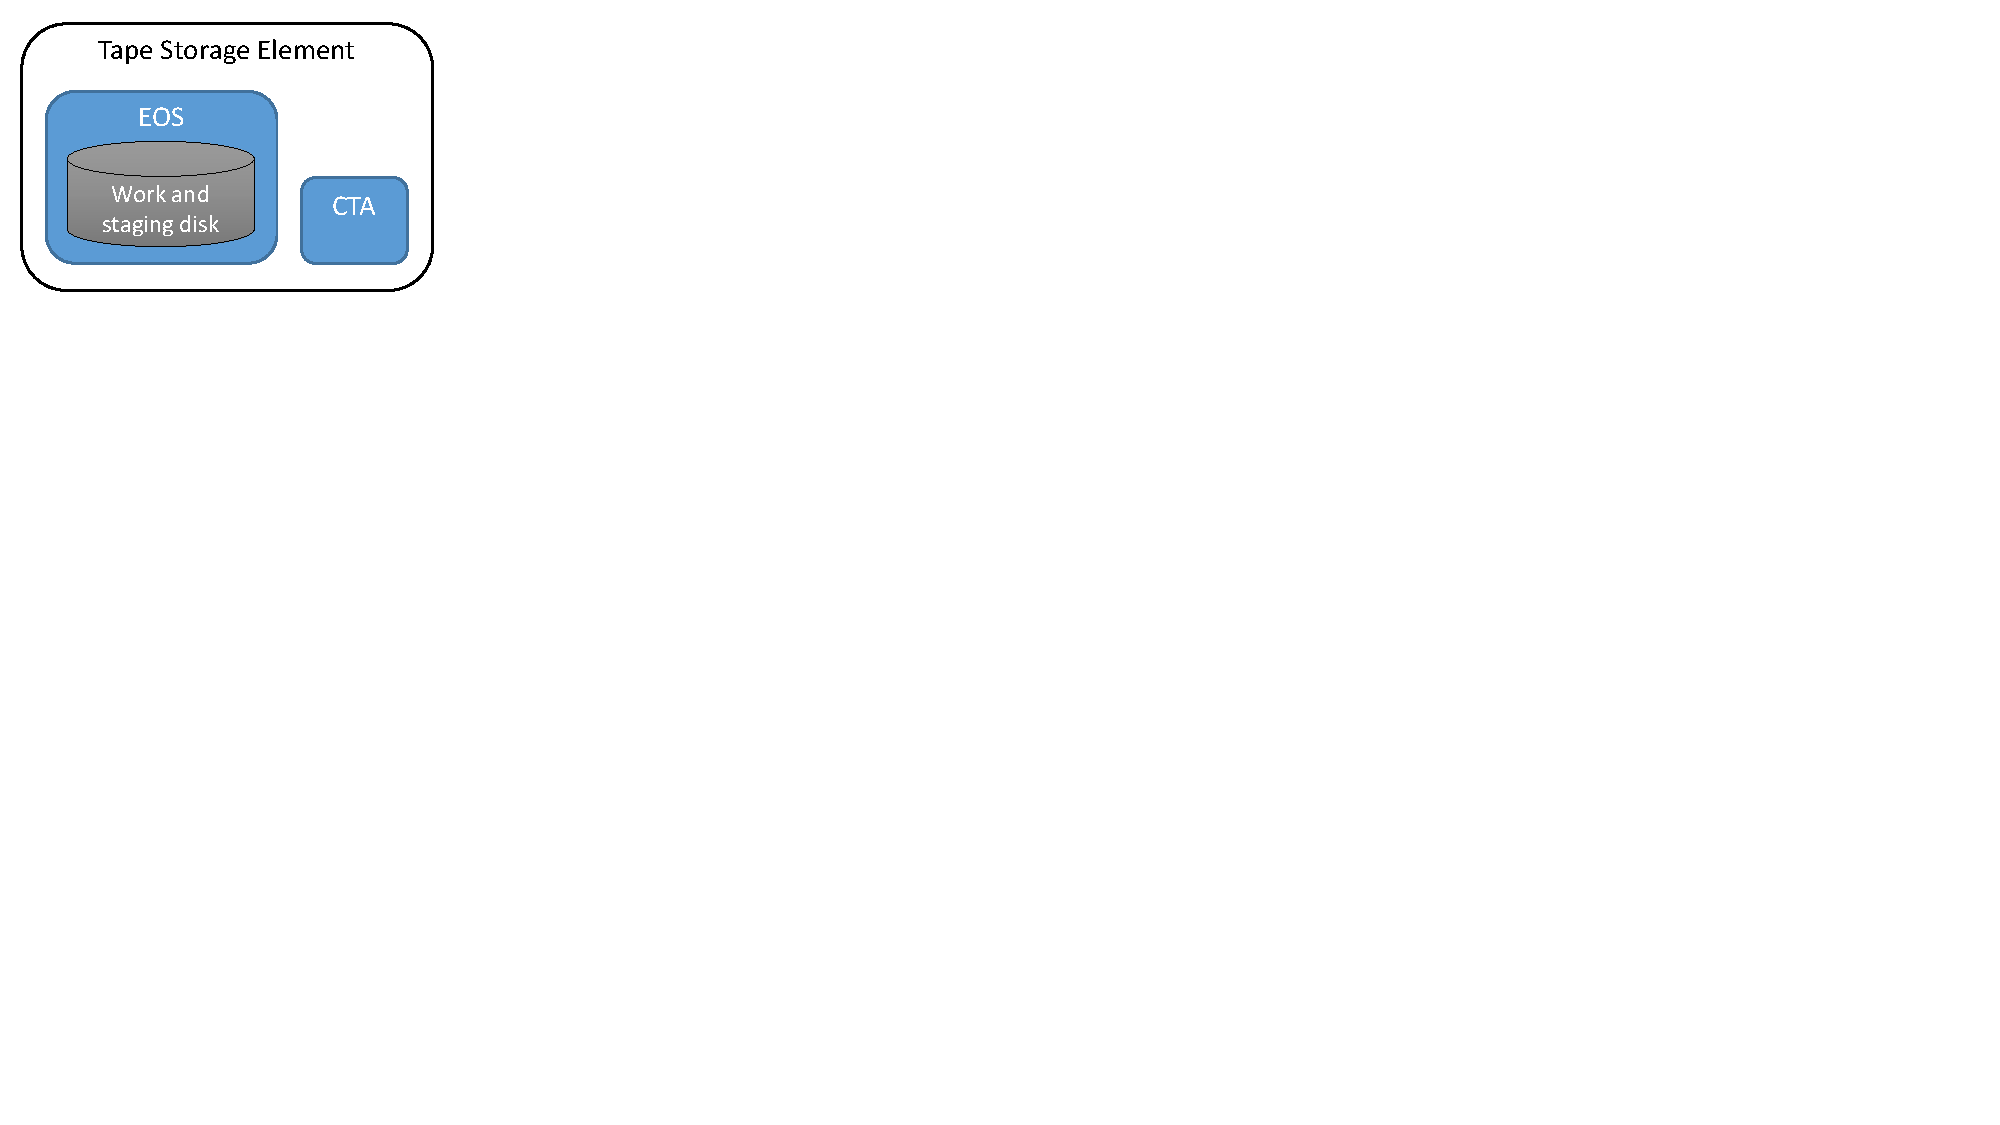
\includegraphics[width=\linewidth,trim=0mm 140mm 0mm 0mm]{EOSTAPE_public_1_pool}
	
	A user would initially create a file in the work pool where they could repeatedly open, modify and close it.  Once the file was completed the user would move it from the work pool to the staging pool in order to have it archived to tape.
	\item Deploy an EOSTAPE Storage Element with a single internal EOS disk pool that uses EOS workflow functionalities to allow a file to be opened and modified many times before having it earmarked for archival to tape.
	
	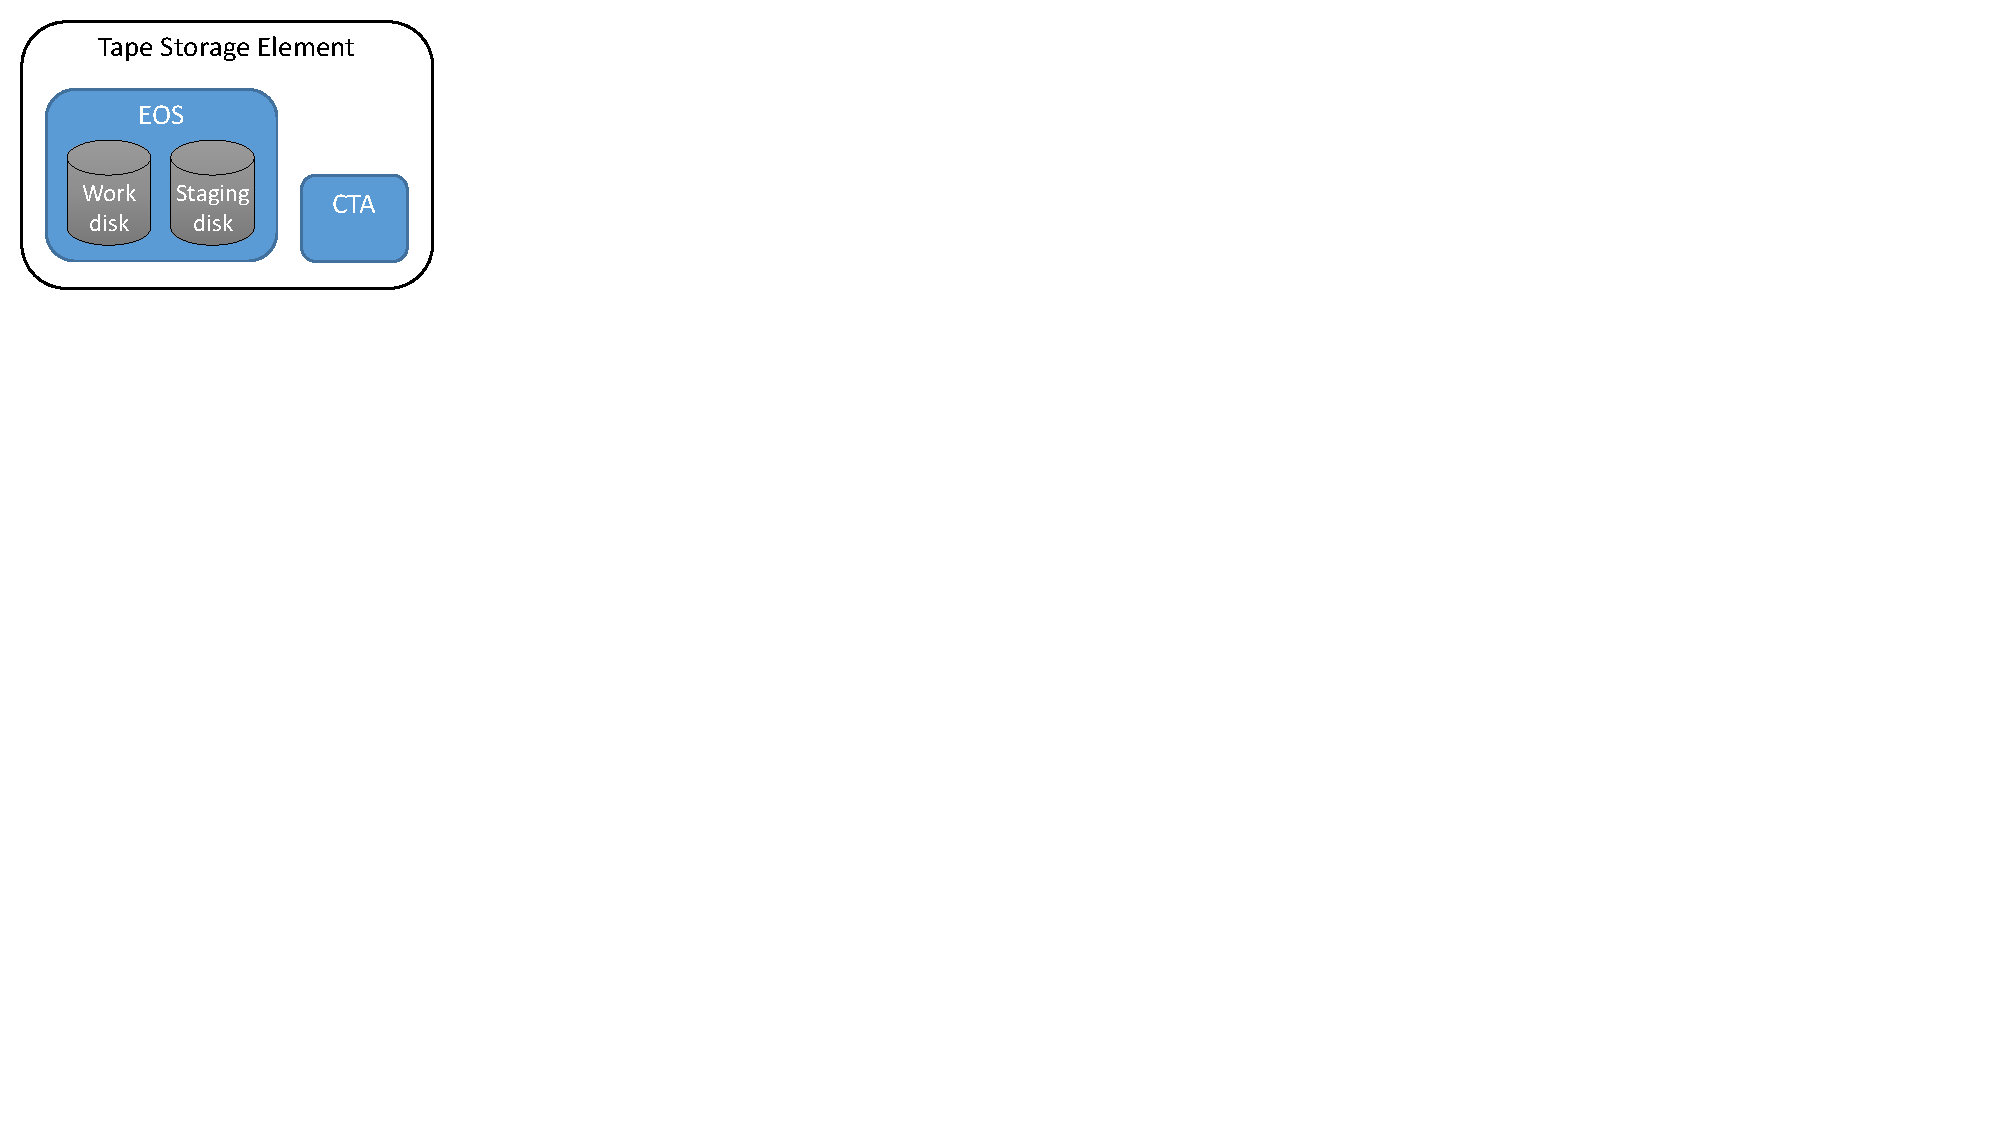
\includegraphics[width=\linewidth,trim=0mm 140mm 0mm 0mm]{EOSTAPE_public_2_pools}
	
	A user would initially create a file without a workflow.  This file could then be modified as many times as the user wishes.  Once the user finished modifying the file they would have it archived to tape by setting its workflow to an "archive to tape" workflow.
\end{itemize}

\newpage
\section{Migrating user files from CASTOR to EOSTAPE}

\subsection{The tape format}

EOSTAPE will use exactly the same tape format as CASTOR.  This will have two significant consequences on the migration of user files from CASTOR to EOSTAPE.  The first and most important consequence will be the fact that only metadata needs to be transferred from CASTOR to EOSTAPE.  There will be no need to copy user files from CASTOR tapes to EOSTAPE tapes.  The second consequence will be the need to preserve the 64-bit numeric identifiers that CASTOR uses to uniquely identify its files independently of the user provided logical names that can be changed many times.

The following diagram illustrates the CASTOR tape format by showing the result of archiving two data files onto the beginning of a tape.  Three files are written to tape for every data file archived.  A header file followed by the data file itself, followed by a trailer file.  The header and trailer files contain metadata describing the data file.  The very first header file of a tape is different from all of the rest because it contains some extra information that describes the tape volume itself.

\begin{tabular}{|c|c|c|c|c|c|}
	\hline
	Volume and header file & Data file 1 & Trailer file & Header file & Data file 2 & Trailer file \\
	\hline
\end{tabular}

Both the header and trailer labels contain a system code field that identifies the creating system and a file identifier field that identifies the data file within the CASTOR namespace.  The file identifier is a 64-bit number written as a hexadecimal string.  When a file is read from tape the file identifier is cross checked to make sure the file being read is in fact the one being requested.  The file identifier is also used by tape operators to facilitate disaster recovery.

The system code field has a length of 13 ASCII printable characters.  The current format of the system code is \texttt{CASTOR} plus the CASTOR base version, for example \texttt{CASTOR 2.1.15}.  When EOSTAPE archives a file to tape it shall use the same format and write EOSTAPE instead of CASTOR for example \texttt{EOSTAPE 1.0}

Tape files must have unique file identifiers that are never reused in order for tape operators to be able to recover files written to tape but accidentally deleted from the archive namespace by users.  A tape operator cannot renter the namespace metadata of a user deleted file if its identifier clashes with that of a newly created file.

The 64-bit CASTOR file identifier will be mapped directly to the archive file identifier of the EOSTAPE Archive File Catalogue (AFC).  The AFC will create new identifiers that will not overlap with the existing CASTOR ones.  It will most probably not be possible to migrate all of the files within CASTOR to EOSTAPE in one instantaneous operation.  A sufficient gap should therefore be purposely introduced between the exiting CASTOR file identifiers and the AFC ones so that CASTOR can continue to create new files whilst the process of migrating files from CASTOR to EOSTAPE is being carried out.

\newpage
\subsection{The granularity of the migration}

A CASTOR tape pool is a logical grouping of tapes and is usually owned by a single Virtual Organisation.  The tapes within a such a pool can be of different hardware types located in different tape libraries.  At a very high-level of abstraction, migrating user files from CASTOR to EOSTAPE will simply consist of transferring the ownership of a tape pool from CASTOR to EOSTAPE.

The architecture of EOSTAPE does not impose any restrictions on the number of tape Storage Elements.  The actual number deployed will be decided by operations.  Assuming that there would be a one to one correspondence between the CASTOR stagers of today and the EOSTAPE tape Storage Elements of tomorrow, then there would be a total of 5 production tape Storage Elements:
\begin{itemize}
	\item EOSTAPE ALICE
	\item EOSTAPE ATLAS
	\item EOSTAPE CMS
	\item EOSTAPE LHCb
	\item EOSTAPE Public
\end{itemize}

Each of these 5 Storage Elements will have its own internal EOS instance.  Transferring the ownership of a CASTOR tape pool to EOSTAPE will actually mean transferring its ownership to the internal EOS instance of one of the above tape Storage Elements and to the Archive File Catalogue (AFC).

\newpage
\section{Orchestrator}
The following diagram shows a high level view of the architecture of the orchestrator by providing an example of how a file would be archived to tape.

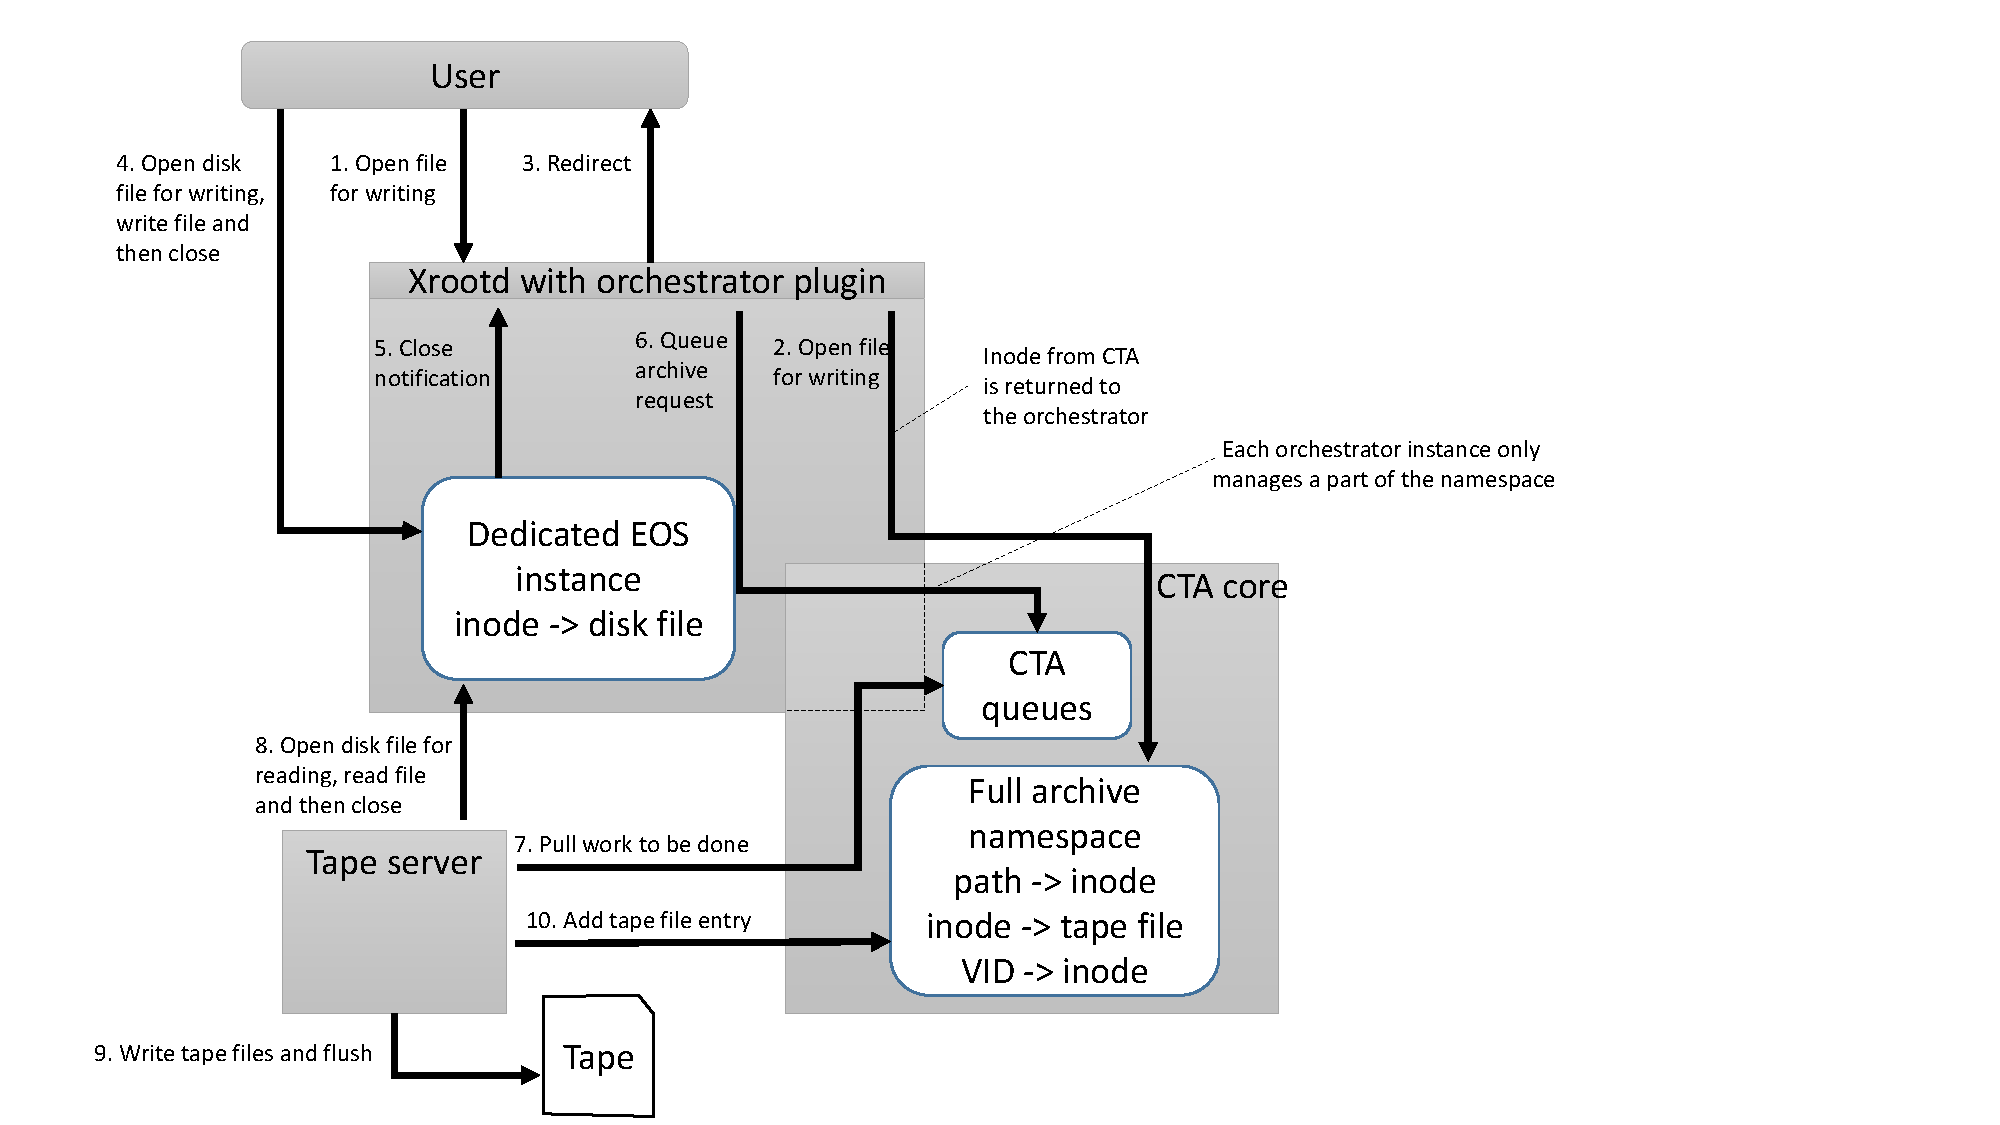
\includegraphics[width=\linewidth]{CTA_orchestrator}

\subsection{Archive a file to tape}
\begin{enumerate}
	\item The user runs a command-line tool to synchronously copy a file from their local disk to the disk staging area (the internal EOS instance) of the tape Storage Element. \\
	\texttt{xrdcp local\_file root://tape\_se\_host//tape\_dir/tape\_file}
	\item The command-line tool connects to the orchestrator and requests \texttt{tape\_file} be opened for writing.
	\item The orchestrator creates \texttt{tape\_file} within the archive namespace and gets the inode of the file back in return.
	\item The orchestrator uses the inode to build a path for the disk copy within the internal EOS instance, for example \texttt{/eos/inodes/12345}.
	\item The orchestrator redirects the command-line tool to the internal EOS instance.
	\item The command-line tool opens and writes the disk copy (\texttt{/eos/inodes/12345}).
	\item The command-line tool successfully completes and returns control to the user.
	\item The internal EOS instance notifies the orchestrator of the successful close.
	\item The orchestrator enqueues an archive request in CTA.
	\item A tape server pulls the archive request from CTA.
	\item The tape server reads the disk copy (\texttt{/eos/inodes/12345}) from the internal EOS instance.
	\item The tape server writes the file to tape.
	\item The tape server updates the tape file entry in the CTA archive namespace.
\end{enumerate}

\subsection{Retrieve a file that is not on disk but is on tape}
\begin{enumerate}
	\item The user runs a command-line tool to synchronously copy the file from the disk staging area (the internal EOS instance) of the tape Storage Element onto their local disk.\\
	\texttt{xrdcp root://tape\_se\_host//tape\_dir/tape\_file local\_file}
	\item The command-line tool connects to the orchestrator and requests \texttt{tape\_file} be opened for reading.
	\item The orchestrator checks for the existence of \texttt{tape\_file} within the archive namespace, and gets the inode of the file back in return.
	\item The orchestrator uses the inode to build a path for the disk copy within the internal EOS instance, for example \texttt{/eos/inodes/12345}.
	\item The orchestrator checks for the existence of the disk copy (\texttt{/eos/inodes/12345}) within the internal EOS instance.
	\item The user is notified that the file does not exist on disk.
\end{enumerate}

An equivalent option is to redirect in all cases and let the client discover that the file is missing in the EOS instance.

\subsection{Prepare a file for access by requesting it be staged to disk}
\begin{enumerate}
	\item The user runs a command-line tool to request the file be staged onto the disk staging area (the internal EOS instance) of the tape Storage Element. \\
	\texttt{xrdfs prepare -s /tape\_dir/tape\_file}
	\item The command-line tool connects to the orchestrator and requests \texttt{tape\_file} be prepared (brought on-line).
	\item The orchestrator checks for the existence of the file within the archive namespace, and gets the inode of the file back in return.
	\item The orchestrator uses the inode to build a path for the disk copy within the internal EOS instance, for example \texttt{/eos/inodes/12345}.
	\item The orchestrator checks that the disk copy (\texttt{/eos/inodes/12345}) does not exist within the internal EOS instance.
	\item The orchestrator enqueues a retrieve job in CTA.
\end{enumerate}

\subsection{Poll for the presence of a file on disk}
\begin{enumerate}
	\item The user runs a command-line tool to poll the orchestrator for the existence of the file on the disk staging area (the internal EOS instance) of the tape Storage Element\\
	\texttt{xrdfs stat root://tape\_se\_host//tape\_dir/tape\_file}
	\item The command-line tool connects to the orchestrator and requests the status of \texttt{tape\_file}.
	\item The orchestrator checks for the existence of the \texttt{tape\_file} within the archive namespace, and gets the inode of the file back in return.
	\item The orchestrator uses the inode to build a path for the disk copy within the internal EOS instance, for example \texttt{/eos/inode/12345}.
	\item The orchestrator queries the internal EOS instance for the existence of the disk-copy (\texttt{/eos/inodes/12345}).
	\item The orchestrator sends the result back to the user.
\end{enumerate}

\subsection{Retrieve a file that has been staged onto disk}
\begin{enumerate}
	\item The user runs a command-line tool to synchronously copy the file from the disk staging area (internal EOS instance) of the tape Storage Element onto their local disk.\\
	\texttt{xrdcp root://tape\_se\_host//tape\_dir/tape\_file local\_file}
	\item The command-line tool connects to the orchestrator and requests \texttt{tape\_file} be opened for reading.
	\item The orchestrator checks for the existence of the \texttt{tape\_file} within the archive namespace, and gets the inode of the file back in return.
	\item The orchestrator uses the inode to build a path for the disk copy within the internal EOS instance, for example \texttt{/eos/inode/12345}.
	\item The orchestrator redirects the command-line tool to the internal EOS instance.
	\item The command-line tool reads the contents of the disk copy (\texttt{/eos/inode/12345}) and writes it to the local disk of the user.
\end{enumerate}

\end{document}
